\documentclass[12pt]{article}
\usepackage[dvipsnames]{xcolor}
\usepackage[10pt]{moresize}
\usepackage[utf8]{inputenc}
\usepackage{latexsym,amsfonts,amssymb,amsthm,amsmath}
\usepackage[letterpaper, portrait, margin=0.7in]{geometry}
\usepackage{parskip}
\usepackage{tkz-euclide}
\usepackage{pgfplots}

\usepackage{hyperref}
\hypersetup{
    colorlinks=true,
    linktoc=all, 
    linkcolor=black,}

\usetkzobj{all}
\newcommand{\abs}[1]{\left| #1 \right|}
\pgfplotsset{compat=1.16}

\theoremstyle{plain}

\newtheorem{theorem*}{Theorem}[subsection]
\newtheorem{theorem}{Theorem}[subsection]
\newtheorem{thm}{\textit{Theorem}}

%      Blackboard bold letters
\newcommand{\bC}{{\mathbb{C}}}
\newcommand{\bN}{{\mathbb{N}}}
\newcommand{\bQ}{{\mathbb{Q}}}
\newcommand{\bR}{{\mathbb{R}}}
\newcommand{\bZ}{{\mathbb{Z}}}
\newcommand{\Mod}[1]{\ (\mathrm{mod}\ #1)}
\newtheorem{definition}{Definition}[subsection]
\newtheorem{lemma}{Lemma}[subsection]
\newtheorem{conjecture}{Conjecture}
\newtheorem{proposition}{Proposition}[subsection]
\newtheorem{example}{Example}[subsection]
\newtheorem{corollary}{Corollary}[subsection]


\newcommand{\de}{\delta}
\newcommand{\ep}{\varepsilon}
\renewcommand{\phi}{\varphi}

\newcommand{\dlim}{\displaystyle\lim\limits}
\newcommand{\dsum}{\displaystyle\sum\limits}
\let\emptyset\varnothing

\DeclareMathOperator{\Dom}{dom}
\DeclareMathOperator{\Img}{img}


\begin{document}

\begin{titlepage}
\begin{center}
    \textbf{\large Math 147  Notes}\\[1ex]
   	\large{Velo.X}\\ 
\end{center}
\end{titlepage}
\newpage

\tableofcontents\label{toc}

\newpage
% line 46
\section{Basics}
	\subsection{The Language of Mathematics}
	Sets: 
	\begin{description}
		\item $x\in X$ ($x$ is an element of $X$)
		\item $y \subseteq X$ ($y$ is a subset of $X$)
		\item X=Y
	\end{description}

	Mathematical Statements are either true or false.

	Combine statements to make new ones. 

	Statement $p$ (true): 

	\begin{itemize}
		\item not: not $p$ (false)

		\item and: $a|b$ and $b|a$

		\item implication: If $p$ then $q$. 
			$\rightarrow$ means $p$ implies $q$, 
			if $p$ is true then $q$ must also be true. 

		\item converse: If $q$ then $p$. $\rightarrow$ 

		\item contrapositive: 
			$p \Rightarrow q$ $\rightarrow$ $\neg q \Rightarrow \neg p$. 
			(the two are equivalent)
	
	        \item $\forall$: e.g. $\forall n \in \mathbb{N}$, 
	        	$n^2+n$ is even. (F)
	        
	        \item $\exists$: e.g. $\exists n \in \mathbb{N}$,
	        	s.t. $n \cdot 0 \neq 0$. (F)
	    \end{itemize}
	
	    Note that the order of the statements matters: 
	    $\forall n \in \mathbb{N}$, 
	    $\exists m \in \mathbb{N}$, s.t. $13|n^2+m^2$. (T)
	
	    $\exists m \in \mathbb{N}$, 
	    $\forall n \in \mathbb{N}$, s.t. $13|n^2+m^2$. (F)
	
	


    \vspace{0.2 in}
    \subsection{Proof}
    \subsubsection{Direct Proof}
			work through to the conclusion
        
        Example: If $x \in \mathbb{R}$, with decimal expansion 
        $x = x_0.\, \,x_1 \, x_2 \, x_3$, $(x_0 \in \mathbb{Z}, 
        x_n \in \{0, 1, 2, 3 \cdots, 9\})$. Say this expansion is eventually 
        periodic, then $\exists \mathbb{N},\, a \in \mathbb{N},\, x_i+d = x$.
        


        \begin{theorem}
            If the decimal expansion of $x$ is eventually periodic, 
            then $x $ is rational.
        \end{theorem}
        \begin{proof}
            Since $x$ has a periodic expansion, we have $N, d \in \mathbb{N}$,
            such that $x_{i+d} = x_i$ for all $i \leq N$. 
            \begin{align*}
                10^{N+d} x &= c. \,\, x_{N+1+d} \,\, x_{N+2+d} \,\, x_{N+3+d}\\
                10^N x     &= b. \,\, x_{N+1}   \,\, x_{N+2}   \,\, x_{N+3} \\
                (10^{N+d} - 10^N)x &= c-b \\
                x &= \frac{c-b}{10^{N+d}-10^N} \in \mathbb{Q}
            \end{align*}
        \end{proof}   
        
        
        \begin{theorem} [\textbf{Pigenhole Principle}]
            If $kn+1$ or more objects are divided into $n$ groups
            then at least $1$ group will contain $\geq k+1$ objects. 
        \end{theorem}
        
        
        \begin{theorem}
            If $x$ is rational, then it has periodic decial expansion. 
        \end{theorem}
        \begin{proof}
            Write $x$ as $\frac pq$, $q\in\mathbb{N}$, $p \in \mathbb{Z}$. 
            (Without loss of generality, $x \geq 0$).

            Divide $10^k$ by $q$, the remainder 
            $r_k \in \{0 , 1 , 2, \cdots, q-1\}$.

            Then $r_0,$ $r_1,$ $r_2,$ $r_3,$ $\cdots,$ $r_q$ 
            $\in$ $\{0, 1, \cdots, q-1\}$,
            By the Pigeonhole Principle, there are $0 \leq i < j \leq q$, 
            so that $r_j = r_q$.
            
            Hence $q$ divides $10^j - rq$ and $10^q - rq$. Therefore $q$ 
            divides $(10^i -ri)-(10^j - rj) = 10^j-10^i = aq$. 
            Therefore: 
            \begin{align*}
                x = \frac pq = \frac{ap}{aq}&=10^{-i} \\
                \frac{ap}{10^j-10^i}&=10^{-i}(b+\frac{r}{10^d-1})\\
                \qquad d = j-i,\,\, 0\leq r< 10^d-1
            \end{align*}
            The expansion of $x$ is eventually periodic because the 
            expansion of $\frac r{10^d-1}$ is eventually periodic.
            let $y$ be a number that has periodic decimal expansion, 
     
     				such that $y = 0. r_{d-1} \,\, r_{d-2} \,\, r_1 
            \,\,r_0\,\,r_{d-1}\,\, r_{d-2}\cdots$
            \begin{align*}
                y &= 0. r_{d-1} \,\, r_{d-2} \,\, r_1 
											 \,\,r_0\,\,r_{d-1}\,\, r_{d-2}\cdots\\
                10y &= r_{d-1} \,\, r_{d-2}\,\, \cdots r_0. r_{d-1} 
                       r_{d-2}\dots\\
                y &= \frac r{10^d-1}
            \end{align*}
            Therefore, $\frac{4}{10^d-1}$ has periodic decimal expansion
            and so does $x$.
        \end{proof}



        \subsubsection{Proof by Contradiction} 
        To prove $(A)$ we can assume $\neg (A)$ and find that it is impossible.
        
        \begin{theorem}
            If $d\geq 2$, $d\in\mathbb{N}$ is not a perfect square 
            then $\sqrt d$ is irrational.
        \end{theorem}
        \begin{proof}
            Find $m \in \mathbb{N}_0$ such that $m^2 < d < (m+1)^2$.
            
            Assume that $\sqrt d$ is rational ($\sqrt d = \frac pq$, 
            $q \sqrt d = p$).

            let $A = \{n \in \mathbb{N} : n\sqrt d \in \mathbb{N}\}$. 
            A is not empty, by Well Ordering Principle, this set
            has a smallest number $a$. 
            \begin{align*}
                m &< \sqrt 3 < m+1 \qquad a\sqrt d \in \mathbb{N} \\
                a & < \sqrt d - m < 1
            \end{align*}
            \begin{align*}
                \text{Let\,\,\,} 
                b &= (\sqrt d - m) a \Rightarrow 0 < b < a\\
                &=a\sqrt d - am  \Rightarrow b \in \mathbb{N}\\
                b\sqrt d &= ad = am\sqrt d \qquad \in \mathbb{N}
             \end{align*}
            so $b \in A$ but $b < a$, contradiction, 
            so $\sqrt d$ is irrational.
        \end{proof}


        \subsubsection {Proof by Induction}
        Given $P(n)$ for $n\geq N_0$ (usually 0 or 1),
        if  $P(n)$ is true and whenever $P(n)$ is true for $n_0\leq n < m$, 
        then $P(m)$ is true.

        \begin{theorem}
            Every $\mathbb{Z}\geq 2$ can be factored
            as a product of 1 and primes.
        \end{theorem}
        \begin{proof}
            Let $P(n)$ be the statement that $n$ is a product of prime numbers.
            
            We knwo that $P(2)$ is true because 2 is a prime.

            Suppose $P(k)$ is true for all $s\leq k\leq n-1$. 
            Consider $P(n)$,

            \setlength\parindent{12pt} Case 1: $n$ is a prime number, 
                and $P(n)$ is true. 

            \setlength\parindent{12pt} Case 2: $p$ is not a prime
                then $n = a\times b$, $1 < a$, $b<n$. 
                Since we assumed that $p(a)$ and $P(b)$ are true,
                so $a = p_1 \cdots p_\alpha$ and $b = q_1 \cdots q_\beta$,
                both product of primes. 
                so $n = p_1 \cdots p_\alpha \cdots q_1 \cdots q_\beta$,
                which is a product of primes.
                Hence by Induction, $P(n)$ is true for all n.\\
        \end{proof}

        \begin{definition}
            The FIBONACCI numbers $F(0) = F(1) = 1$, 
            and $F(n) = F(n-1) = F(n-2)$ for $n\geq 2$. 
            (1, 1, 2, 3, 5, 8 ...).

           $\phi = \frac{1+\sqrt 5}2$      \qquad  \qquad
           $\frac 1 {\phi} = \frac{\sqrt 5-1}2$ 

           $\phi ^ 2= \frac{3+\sqrt 5}2= 1+\phi$ \qquad 
           
           $\frac1 {\phi ^2} = 1 -\frac1 {\phi}$ \\
        \end{definition}

        \begin{theorem}
            Let $F(n)$ be a Fibonacci Sequence, 
            then $F(n) = \frac{\phi^{n+1} -(\frac{-1}{\phi})^{n+1}}{\sqrt 5}$
        \end{theorem}
        \begin{proof}
            Let $P(n)$ be that 
						$F(n) = \frac{\phi^{n+1} -(\frac{-1}{\phi})^{n+1}}{\sqrt 5}$.

            $P(0) = \frac{\phi - (\frac{-1}{\sqrt \phi})^1}{\sqrt 5} = 1$, 
            $P(n)$ is true.

            $P(1) = \frac{\phi ^2 -(\frac{-1}{\phi})^2}{\sqrt 5} = 
            \frac{1+\phi-\frac1{\phi^2}{\sqrt 5}}{\sqrt 5}=1$, 
            so $P(1)$ is true.

            Assume $P(k)$ is true for $0\leq k < n$, $n\geq 2$. 
            \begin{align*}
                F(n)&= F(n-1)+F(n-2)\\
                    %
                    &= \frac{\phi ^{n-1+1} -(\frac{-1}{\phi})^{n-1+1}}{\sqrt 5}
                    + \frac{\phi ^{n-1}-(\frac{-1}{\phi})^{n-1}}{\sqrt 5}\\
                    %
                    &=\frac1{\sqrt 5} (\phi^{n-1} (\phi +1) - 
                    (\frac{-1}{\phi})^{n-1})(\frac{-1}{\phi}+1))\\
                    %
                    &=\frac1{\sqrt 5}\cdot (\phi^{n+1} \cdot\phi ^2 - 
                    (\frac{-1}{\phi})^{n-1}\cdot (\frac{-1}{\phi}) ^ 2)\\
                    %
                    &=\frac{\phi^{n+1} - (\frac{-1}{\phi})^{n+1}}{\sqrt 5}
            \end{align*}
            hence, by induction, $P(n)$ is true for all $n\geq 0$.
        \end{proof}
   


    \subsection{Real Numbers}
    A real number $x$ has an infinite decimal expansion. 

    $x = x_0.x_1 x_2x_3 \cdots$, 
    $x_0\in \mathbb{Z}, \,\,x{i}\in\{0 , 1 , 2, \cdots 9\}$,\,\, $i \geq 1$.\\\\
    Think "$\sum_{n=1}^{\infty} \frac{x^n}{10^n} = 1$" as a formal name for $x$.\\\\
    \textbf{Example:}

    $-1.25 = -1.2500000...$

    Some real numbers have two names. Ex : $1.000\cdots = 0.999\cdots$

    \vspace{0.5in}

    \subsection{Order}
    The real number $\mathbb{R}$ is an ordered field. 

    If $x, y \in \mathbb{R}$, then $x < y \land x=y \land x>y$. 
    
    If $x \neq y$ then the decimal expansion diverges at some point. 
    
    If $x < y$, then there is $r\in \mathbb{Q}$ with a finite expansion 
    such that $x < r< y$. 
    
    This says that the rationals are dense in $\mathbb{R}$. 

    \begin{theorem*}{Archimedean Property}
        If $x\in\mathbb{R}$ and $0\leq x \leq 10^{-n}$ 
        for all $n\geq 1$. then x=0.
    \end{theorem*}
    \begin{proof}
        Let $x = x_0. \,\, x_1 x_2 x_3\cdots$.
        If $0 < x$, then $x\geq 0$, $x = 0.000\cdots x_n$, 
        then $x \geq 0 > 10^{-n-1}$,
        so the only real number satisfying the hypothesis is 0.
    \end{proof}
    
    \newpage

\section{Sequence}
    \subsection{Limits}
    $\dlim_{n\to\infty} x_n = L$
    
    {\color{Brown}
    \textbf{Example:} 
    \begin{itemize}
        \item $a_n = \frac1n$, $n\geq 1$  
            $\Rightarrow \dlim_{n\to\infty} a_n = 0$
        \item $a_n = 0$ $\Rightarrow \dlim_{n\to\infty} a_n = 0$
        \item $0$ , $1$, $0$, $\frac12$, $0$, $\frac13$ $\cdots$
        $\Rightarrow \dlim_{n\to\infty} a_n = 0$
        \item $1$, $-1$, $1$, $-1$, $1$, $\cdots$ $\Rightarrow$ limit D.N.E.
    \end{itemize}}
    \bigskip
    \begin{definition}
        $\dlim_{n\to\infty} x_n=L$ mean for every $\epsilon >0$, 
        exists $N$ so that $\abs{a_n-L} < \epsilon$ for all $n\geq N$.

        $\forall\,\, \epsilon > 0$ , $\exists N$, 
        $\forall n\geq N$, $\abs{a_n-L} < \epsilon$.
    \end{definition}

    {\color{Brown}
    \textbf{Example 1:
        $-1$, $0$, $\frac12$, $0$, $-\frac13$, $\cdots$, 
        $   
            a_n=
            \begin{cases}
                \frac{(-1)^k}k, & n = 2k-1\\
                0,   &n = 2k \\
                \end{cases}
        $}

        If $\epsilon > 0$, 
        there is $10^{-k} < \epsilon$.

        Let $N = 2\cdot 10^k$, 
        if $n\geq N$, and $n$ is even, then $a_n = 0$, 
        $\abs{a_n - 0} = 0<\epsilon$, 
        
        if $n$ is odd, let $N = \frac 2{\epsilon}$, 
        then $a_n = \pm \frac1{k}$, 
        $\abs{\pm\frac1k - 0} = \frac1k \leq \frac1N<\frac{\epsilon}2$.\\

    \textbf{Example 2: $-1$, $1$,  $-1$, $1$, $\cdots$, $a_n = (-1)^n$}

        $\dlim_{a_n} \neq L$ means for $\exists \epsilon_0 > 0$
        and $\abs{a_{n_k}-L}\geq \epsilon_0$.

        Take $\epsilon =1$,

        if $L > 0$, since $a_{2n+1} = -1$, 
        $\abs{a_{2n+1} -L} = \abs{-1-L} > 1=\epsilon$.
        
        if $L \leq 0$, since $a_{2n} = 1$,
        $\abs{a_{2n} -L} = \abs{1-L} \geq 1=\epsilon$.
                
        Hence no limit exists.\\
        
    \textbf{Example 3: Let $a_n = \dfrac1{2+\dfrac1{2+\dfrac1{2+\cdots}}}$, with $n$ 2s. }
        
        $a_1 = \frac12$, $a_2 = \frac1{2+\frac12}=\frac25$ $\cdots$, 
        $a_{n+1} = \frac1{2+a_n}$, $n\geq1$.

        Suppose the limit exists, $\dlim_{n\to\infty} a_n = L$, 
        then $L = \dlim_{n\to\infty} a_n = \dlim_{n\to\infty} a_{n+1}
        = \frac1{2+L}$.

        Solve for $L$, $L^2+2L-1 = 0 \Rightarrow L = -1\pm\sqrt2$.

        Since $a_n\geq0$, hence $L\geq 0$ and $L= -1+\sqrt 2$.}
        
    \newpage
    {\color{Blue}
    \begin{theorem}{\textbf{Squeeze Theorem} \\}
        If $a_n \leq x_n\leq b_n$, and 
        $\dlim_{n\to\infty} a_n= L = \dlim_{n\to\infty}b_n$, 
        then $\dlim_{n\to\infty} x_n = L$. 
    \end{theorem}
    \begin{proof}
        let $\epsilon > 0$, since $\dlim_{n\to\infty} a_n = L$, 

        $\exists \,\,N_1$, $n\geq N_1$ $\Rightarrow \abs{a_n-L} < \epsilon$,
        so $L-\epsilon < a_n< L+\epsilon$.

        $\exists \,\,N_2$, $n\geq N_2$ $\Rightarrow \abs{b_n-L} < \epsilon$,
        so $L-\epsilon < b_n< L+\epsilon$.
        
        Let $N = \max\{N_1, N_2\}$, $n\geq N$ 
        $\Rightarrow L -\epsilon < a_n\leq x_n\leq b_n<L+\epsilon$ 
        $\Rightarrow \abs{x_n-L}<\epsilon$ so $\dlim_{n\to\infty} x_n=L$.
    \end{proof}}

    \begin{theorem}
        A sequence can and can only have one limit.
    \end{theorem}
    \begin{proof}
        Assume a contradiction that $\dlim_{n\to\infty} a_n = L$
            and $\dlim_{n\to\infty} a_n = M$, $M>L$.

        Let $\epsilon = \frac{\abs{L-M}}2$, since $\exists N$, $\forall n\geq N$,
        $\abs{x_n-L}<\epsilon$. Hence 
        $L-\epsilon < x_n < L+\epsilon =L+\frac{M-L}2 =\frac{L+M}2<M$ 
        Contradiction.                
    \end{proof}

    \begin{proposition}
        Suppose $(a_n)_{n=1}^\infty$ and $(b_n)_{n=1}^\infty$ are sequences
        and that $\dlim_{n\to\infty} a_n = L$ and $\dlim_{n\to\infty} b_n = M$, 
        then
        \begin{enumerate}
            \item of $k \in\mathbb{R}$, $\dlim_{n\to\infty} k \cdot a_n = k\cdot L$\\
            \begin{proof}
                We know that there is an $N$ such that for all $n\geq N$, 

                $\abs{a_n-L}<\frac{\epsilon}{\abs{k^2+1}}$, 

                therefore, $\abs{ka_n-kL}=\abs{k}\abs{a_n-L}
                <\abs{k}\abs{\frac{\epsilon}{k^2+1}}<\epsilon$,

                hence, by defnition of limit, $\dlim_{n\to\infty} ka_n = kL$.
            \end{proof}

            \item $\dlim_{n\to\infty} a_n\pm b_n = L\pm M$
            \begin{proof}
                Let $\epsilon > 0$, 
                $\abs{a_n+b_n-L-M} \leq \abs{a_n-L}+\abs{b_n-M}$.

                Since $\dlim_{n\to\infty} a_n = L$, $\exists N_1$, 
                $n\geq N_1 \Rightarrow \abs{a_n -L }< \frac{\epsilon}2$

                and $\dlim_{n\to\infty} b_n = M$, so $\exists N_2$, 
                $n\geq N_2 \Rightarrow \abs{b_n -L }< \frac{\epsilon}2$

                Take $N = \max\{N_1, N_2\}$, so if $n\geq N$, then both
                are true.
                
                $\therefore \abs{a_n+b_n-L-M}\leq \abs{a_n-L}+\abs{b_n-M}
                <\frac{\epsilon}2 + \frac{\epsilon}2 = \epsilon$

                $\therefore \dlim_{n\to\infty} a_n+b_n = L+M$\\
            \end{proof}
            
            \item $\dlim_{n\to\infty} a_n b_n = LM$
            \begin{proof}
                Let $\epsilon>0$, since $\dlim_{n\to \infty} a_n=0$ 
                and $\dlim_{n\to \infty} b_n = 0$,

                there is $N_1$ such that for all $n\geq N_1$, $\abs{a_n-L}<\frac{\epsilon}{2\abs{b_n^2+1}}$ 
                
                and there is $N_2$ such that  for all $n\geq N_2$, $\abs{b_n-L}<\frac{\epsilon}{2\abs{L^2+1}}$
                
                therefore, let $N=\max{N_1, N_2}$, for all $n\geq N$, we have 
                \begin{align*}
                    \abs{a_nb_n-LM} &= \abs{a_nb_n-b_nL+b_nL-LM}\\
                    &=\abs{b_n(a_n-L)+L(b_n-M)}\\
                    &\leq \abs{b_n}\abs{a_n-L}+\abs{L}\abs{b_n-M}\\
                    &<\abs{b_n}\cdot \frac{\epsilon}{2\abs{b_n^2+1}}+\abs{b_n}\cdot \frac{\epsilon}{2\abs{L^2+1}}\\
                    &<\frac{\epsilon}2+\frac{\epsilon}2
                    &=\epsilon
                \end{align*}
            
                Hence, by definition of limit, $\dlim_{n\to \infty} a_nb_n=LM$.
            
            \end{proof}
            
            \item if $M \neq 0$, then $\exists\,\, N$, s.t. 
                    $\forall\,\, n\geq N$, $b_n\neq 0$, 
                    $\dlim_{n\to\infty} \frac{a_n}{b_n} = \frac LM$
            \begin{proof}
                Take $\epsilon = \frac{\abs M}2>0$, find $N_1$, $n\geq N_1$
                \begin{align*}
                    \abs{b_n-M} &< \epsilon = \frac{\abs M}2\\ 
                    \abs{b_n} &= \abs{M-(M-b_n)} \geq \abs{M}-\abs{M-b_n}\\
                    &>\abs{M}-\frac{\abs{M}}2 = \frac{\abs{M}}2 \neq 0
                \end{align*}
                Hence $b_n \neq 0$ if $n\geq N$, and $\frac{a_n}{b_n}$ is defined.

                Estimate:
                \begin{align*}
                    \abs{\frac{a_n}{b_n} -\frac LM} 
                    =&\abs{\frac{a_n\cdot M -b_n\cdot L}{b_n\cdot M}}\\
                    =&\abs{\frac{a_n\cdot M + LM -LM-b_n\cdot L}{b_n\cdot M}}\\
                    \leq &\frac{\abs{a_n-L}\abs{M} + \abs{M-b_n}\abs{L}}
                    {\frac{\abs{M}}2 + \abs{M}}\\
                    =&\frac{\abs M}2 \cdot \abs{a_n-L} + 
                    \frac{\abs{2L}}{M^2} \cdot\abs{M-b_n}
                \end{align*}
                Take $\epsilon_1 = \frac{\epsilon\cdot \abs{M}}4$, so 
                $\frac2{\abs{M}} \cdot \epsilon_1 = \frac{\epsilon}2$. 
                Since $\dlim_{n\to\infty} a_n=L$, $\exists N_2$, s.t. 
                $\forall n \geq N_2 \Rightarrow \abs{a_n-L} 
                < \epsilon_1= \frac{\epsilon\cdot \abs{M}}4$. 
                
                Take $\epsilon_2 = \frac{\epsilon\cdot M^2}{4\cdot\abs{L}}$, so 
                $\frac{2\abs{L}}{M^2} \cdot \epsilon_2 = \frac{\epsilon}2$. 
                Since $\dlim_{n\to\infty} b_n=M$, $\exists N_3$, s.t. 
                $\forall n \geq N_2 \Rightarrow \abs{b_n-M} 
                < \epsilon_2= \frac{\epsilon\cdot M^2}{4\abs{L}}$. 

                Let $N = \max\{N_1, N_2, N_3\}$, for $n\geq N$, means that 
                \begin{align*}
                    \abs{\frac{a_n}{b_n}-\frac LM} &< 
                    \frac2{\abs{M}}\abs{a_n-L} + \frac{2\abs{L}}{M^2}\cdot \abs{b_n-M}\\
                    &<\frac2{\abs{M}}\cdot\frac{\abs{M}}4\cdot\epsilon+
                    \frac{2\abs{L}}{M^2}\cdot\frac{M^2}{4\abs{L}}\cdot\epsilon\\
                    &=\frac{\epsilon}2+\frac{\epsilon}2 = \epsilon
                \end{align*}                    
            \end{proof}
        \end{enumerate} 
    \end{proposition}
    
    
    
    \vspace{0.5 in}
    \subsection{Upper and Lower Bounds}
    \begin{definition}
        If $\emptyset \neq S \subseteq \mathbb{R}$. 
        
        If S is bounded above. ($\exists M$, $\forall s \in S$, $S \leq M$),
        then the least upper bound, or supremum
        is the smallest possible upper bound, written as \textbf{$\sup S$}. 

        Similarly, if S is bounded below, the greatest lower bound or infinium, 
        written as \textbf{$\inf S$}.
    \end{definition}

    {\color{Brown}
    \textbf{Example:} 
    \begin{itemize}
        \item $S=\{2, e, \pi, 4, 17, \frac{37}{\sqrt {47}} \}$, $\inf S = 2$, $\sup S = 17$.
                * when finite set, $\inf S = \min$, $\sup S = \max$.
        \item $S =\{x\in\mathbb{Q} : x^2 < 2\}$, $\sup S =\sqrt2$, $\inf S = -\sqrt 2$.
        \item $S =\{\sin\,\, n : n\in\mathbb{N}\}$, $\sup S = 1$, $\inf S = -1$\\
    \end{itemize}}

    {\color{Blue}
    \begin{theorem}\textbf{Least Upper Bound Principle}\\
        If $S \subseteq \mathbb{R}$ is bounded above, then $S$ has a least 
        upper bound $\sup S$; if $S \subseteq \mathbb{R}$ is bounded below, 
        then $S$ has a greatest lower bound $\inf S$.
        It suffices to prove one statement.
    \end{theorem}
    \begin{proof}
    	Pick $a_0 $ which is a lower bound for $S$, $a_0+1$ is not a lower bound.
        Pick $S_0 \in S$, $s_0 < a_0+1$ (witness).

        Pick $a_1 = \{0, 1, 2, \cdot , 9\}$, such that $a_0.\,a_1$ is a lower bound but
        $a_0. (a_1+1)$ is not. pick $s_1<a_0.\,\, a_1+0.1$.

        Proceed recursively, at stage $n$ we have $a_0. a_1\,\,a_2\,\,a_3\,\,\cdots a_n$
        as a lower bound and $a_0. a_1\,\,a_2\,\,a_3\,\,\cdots a_n + \frac1{10^n}$ is not.
        
        Again split into $10$ pieces,then choose $a_{n+1} \in \{0, 1, 2, \cdots, 9\}$, 
        so $a_0. a_1  a_2  \cdots a_n a_{n+1}$ is a lower bound
         and $a_0. a_1a_2\cdots a_n a_{n+1}+\frac1{10^{n+1}}$ is not
        and pick witness $s^{n+1} < a_0. a_1a_2\cdots a_na_{n+1}+\frac1{10^{n+1}}$.

        Let $s\in S$, then $s\geq a_0. a_1 a_2 a_3\cdots a_n$ for every $n$.
        Therefore $S \geq \dlim_{n\to\infty} a_0. a_1 a_3 a_4 \cdots a_n = L$, 
        so $L$ is a lower bound of S. 

        Suppose $L_1 > L$, $L_1 - L >0$. Since $\mathbb{R}$ is Archimedean, so 
        there $\exists N$, $L_1 \geq L+\frac1{10^N}\geq a_0.a_1a_2\cdots a_n+\frac1{10^N}$.

        But there is $s_N \in S$ $S_N< a_0. a_1\cdots a_N+\frac1{10^N} \leq L_1$,
        therefore, $L1$ is not a lower bound, therefore $L=\inf S$.
    \end{proof}}

    \begin{lemma}
        $\inf S = -(\sup (-S))$ \quad and \quad $\sup S = -(\inf (-S))$
    \end{lemma}

    \begin{definition}
        A sequence $(a_n)_{n=1}^{\infty}$ is monotone increasing if 
        $a_n\leq a_{n_1}$, and strictly increasing if $a_n<a_{n+1}$.
    \end{definition}

    {\color{Blue}
    \begin{theorem}{\textbf{Monotone Convergence Theorem}}\\
        If $(a_n)_{n=1}^{\infty}$ is monotone increasing and bounded above, 
        then $\dlim_{n\to\infty} a_n$ exists.
    \end{theorem}

    \begin{proof}
        Let $(a_n)_{n=1}^\infty$ be a monotone increasing sequence. 
        Then by the LUBP, $\exists L = \sup \{a_n, n\geq 1\}$ $a_n\leq L$ for all $n\geq 1$.

        Let $\epsilon > 0$, then $L-\epsilon$ is not an upper bound. 
        $\therefore \exists N$, $L-\epsilon < a_N$.

        Since for $n\geq N$, $L-\epsilon < a_N\leq a_n \leq L$.
        Therefore $0<L-a_n<L-(L-\epsilon)=\epsilon$, so $\abs{L-a_n} < \epsilon$.
    \end{proof}}

    {\color{Brown}\textbf{Example 1: Let $a_1 = 1$ and $a_{n+1} = \sqrt{2+\sqrt {a_n}}$ for $n\geq 1$.
    Find limit for $a_n$.}

    Claim: $a_n$ is monotone increasing. $a_n<a_{n+1}$

    $a_2 = \sqrt {2+\sqrt 1} > a_1$, proceed by induction, 
    if $a_{n-1}<a_n$, then $a_{n+1} = \sqrt {2+\sqrt {a_n}}> \sqrt {2+\sqrt {a_{n-1}}}=a_n$
    Hence by induction, $a_n> a_{n-1}$ for all $n$.

    Claim: $a_n\leq 2$ for all $n$.
    
    First, $a_1=1<2$. Assume $a_n\leq 2$, 
    then $a_{n+1} = \sqrt {2+\sqrt {a_{n}}}<\sqrt {2+2}=2$. 
    Hence by indcution, $a_n<2$ for all $n$.

    Therefore, $a_n$ is monotone increasing and bounded above, 
    and by Monotone Convergence Theorem, $\dlim_{n\to\infty} a_n=L$ exists.
        
    $L = \dlim_{n\to\infty} a_n = \dlim_{n\to\infty} a_{n+1} 
    = \dlim_{n\to\infty} \sqrt{2+\sqrt{a_n}}=\sqrt{2+\sqrt L}$

    $L^4-4L^2-L+4=0$, solve for L, $L = 1$ or $L = 1$ $L = 1.8312$.

    Since $L \geq a_2=\sqrt 3$, $L\neq 1$, so $L=1.8312$.\\
    
    }

    \begin{proposition}
        If $\dlim_{n\to\infty} a_n=L$ and $(a_{n_i})_{i=1}^{\infty}$ is
        a subsequence, then $\dlim_{n\to\infty} (a_{n_i})_{i=1}^{\infty} = L$. 
    \end{proposition}
    \begin{proof}
        $\dlim_{n\to\infty} a_n= L$ means that there exists 
        $N$ s.t. $n\geq N \Rightarrow \abs{a_n-L} < \epsilon$

        If $i\geq N$, then $n_i\geq i \geq N \Rightarrow 
        \abs{a_{n_i}-L} < \epsilon$
        
    \end{proof}

    \begin{proposition}
        If $\dlim_{n\to\infty} a_n=L$, then $a_n$ is bounded. 
    \end{proposition}
    \begin{proof}
        Let $\epsilon = 1$, Find $N$ s.t. $n\geq N \Rightarrow \abs{a_n-L}<1$
        
        $\therefore L-1<a_n<L+1$,

        $\therefore \abs{a_n}\leq \abs L+1$

        Let $R =\max\{\abs{L}+1, \abs{a_1}, \abs{a_2}\cdots \abs{a_N-1}\}$,
        $\therefore \abs{a_n}\leq R$ for all $n\geq 1$.
    \end{proof}

    {\color{Blue}
    \begin{theorem}\textbf{Bolzano-Weierstrass Theorem}\\
        If $(a_n)_{n=1}^\infty$ is a bounded sequence of real numbers,
        then it has a convergent subsequence. 
    \end{theorem}
    \begin{proof}
        Let $a_n$ be a sequence bounded by $B$, thus the interval
        $I=[-B, B]$ contains the whole infinite sequence. 

        Then of the interval $[-B, 0]$ and $[0, B]$, one of these halfs must 
        contain infinitely many elements of $a_n$, let it be $I_2$.

        Similarly, divide $I_2$ into two closed intervals of length $\frac{B}2$,
        and choose the interval $I_3$ of the two which contains 
        infinitely many elements of $a_n$. 

        Again divide $I_3$ into two closed intervals of length $B/4$ 
        and choose the interval $I_4$ of the two which contains 
        infinitely many elements of $a_n$.

        Therefore we have intervals $I_1$ to $I_k$ in which the 
        length of $I$ decreases as $k$ increases. $I_{k-1} \subset I_k$
        
        Let the left endpoint of $I_k$ be $l_k$ 
        and the right endpoint of $I_k$ be $r_k$.
        Observe that  $l_k\leq l_{k+1}<r_{k+1}<r_k\leq r_{k+1}$.

        Hence $l_k$ is a increasing sequence that is bounded by 
        $r_1$ and $r_k$ is a decreasing sequence which is bounded by $l_1$.

        Hence by monotone convergence theorem, 
        there is $\dlim_{k\to\infty} l_k = L$ and $\dlim_{k\to \infty} r_k = M$.
        
        Since the length of $I_k$ = $\frac B{2^{k-2}}$, 
        hence $M-L=\dlim_{k\to\infty} r_k-l_k = 
        \dlim_{k\to\infty} \frac{B}{2^{k-2}} = 0$.

        Therefore, $M=L$.

        Choose a increasing sequence $a_{n_k}$ that $a_{n_k}$ belong to $I_k$,
        This is possible because each $I_k$ contains infinitely many elements of $a_n$
        and $n_{k-1}$ only fnitely many have index at most $n_{k-1}$. 

        Then $l_k\leq a_{n_k}\leq r_k$, by Squeeze Theorem, 
        $\dlim_{k\to\infty}a_{n_k} = L$.\\
    \end{proof}}


    \begin{definition}
        A \textbf{Cauchy Sequence} is a sequence $(a_n)_{n=1}^\infty$ that
        if $\epsilon > 0$, $\exists \,\, N$ s.t. if $m, n \geq N$, 
        then $\abs{a_n - a_m} < \epsilon$.\\
    \end{definition}

    \begin{proposition}
        Every convergent sequence of real numbers are Cauchy.

        i.e. Let $(a_n)^{\infty}_{n=0}$ be a sequence converging to $L$.
        For every $\epsilon>0$, there is an $N$ such that for all $m, n>0$
        $\abs{a_n-a_m}<\epsilon$.
    \end{proposition}
    \begin{proof}
        Let $\epsilon>0$, and use the value $\frac{\epsilon}2$. 
        
        Then by the definition of limit, there is an $N_1$, such that for all
        $n>N_1$, $\abs{a_n-L}<\frac{\epsilon}2$, 
        
        and so $\abs{a_n-a_m}=\abs{a_n-L+L-a_m}
        \leq \abs{a_n-L}+\abs{a_m-L}<\frac{\epsilon}2+\frac{\epsilon}2=\epsilon$ 

    \end{proof}

    \begin{proposition}
        Every Cauchy sequence is bounded.
    \end{proposition}
    \begin{proof}
        Let $(a_n)^{\infty}_{n=0}$ be a Cauchy sequence, 
        
        then there exists $N$ such that 
        for all $n\geq N$, $\abs{a_n-a_N}<1$.

        It follows that the sequence is bounded by $\max\{\abs{a_1}, \abs{a_2},\cdots, \abs{a_N}+1\}$
    \end{proof}

    \begin{definition}
        A subset $S\subseteq \mathbb{R}$ is \textbf{complete} if a Cauchy Sequenece
        $(a_n)_{n=1}^\infty$ with $a_n\in S$ has a limit 
        $\dlim_{n\to\infty} a_n=L \in S$. \\
    \end{definition}

    {\color{Blue} \begin{theorem}\textbf{Completeness Theorem}\\
        $\mathbb{R}$ is complete. i.e. every Cauchy Sequence of $\mathbb{R}$ converges to $\mathbb{R}$.
    \end{theorem}

    \begin{proof}
        Let the sequence be $(a_n)^{\infty}_{n=0}$. 

        By Proposition 2.2.4, Cauchy Sequences are bounded. 

        Therefore, by Bolzano-Weierstrass Theorem, there is a 
        subsequence $a_{n_k}$ which has $\dlim_{k\to\infty} a_{n_k} = L$.
        
        Hence, there exists an $K$ such that for all $k>K$,
        $\abs{a_{n_k}-L}<\frac{\epsilon}2$.
        
        Since this is a Cauchy sequence $N$ such that for all $n, m>N$, 
        $\abs{a_n - a_m} < \frac{\epsilon}2$. 

        Pick $k>K$ such that $n_k>N$, then for all $n > N$, 
        
        $\abs{a_n-L}\leq \abs{a_n-a_{n_k}}+\abs{a_{n_k}-L}
        <\frac{\epsilon}2 +\frac{\epsilon}2=\epsilon$.

        Hence $\dlim_{n\to\infty} a_n = L$. 
    \end{proof}}

    \newpage

\section{Function}
	\begin{definition}
	For $A, B$ sets, $f: A \to B$ is a function if for each $A\in B$, 
    a value for $f(a) \in B$ is assigned by some rule. \\
	\end{definition}

	\begin{definition}
		Given two nonempty sets $A$ and $B$, a function $f$ from $A$ to $B$ is a 
		subset of $A \times B$, denoted $G(f)$, so that
		\begin{enumerate}
			\item for each $a\in A$, there is some $b\in B$ so that $(a,b) \in G(f)$,
			\item for each $a\in A$, there is only one $b\in B$ so that $(a,b) \in 
				G(f)$.
		\end{enumerate}
		That is for each $a\in A$, there is exactly one elements $b\in B$ with 
		$(a,b)\in G(f)$. We then write $f(a)=b$. A concise way to specify the 
		function $f$ and the sets $A$ and $B$ all at once is to write $f:A\to B$.
		We call $G(f)$ the graph of the function $f$. 

		The property of a subset of $A\times B$ that makes it the graph of a 
		function is that $\{b \in B : (a,b) \in G(f)\}$ has precisely one element
		for each $a\in A$.

		We call $A$ the domain of the function $f: A\to B$ and $B$ is the condomain.
		The range of the function is $Ran(f):=\{b\in B : b= f(a)$
		for some $a\in A \}$.\\
	\end{definition}
    
  {\color{Brown}
  	Example: 
    \begin{itemize}
        \item $f: \mathbb{R} \backslash \{0\} \to \mathbb{R}\backslash \{0\}$ 
        	by $f(x)= \frac1x$
        \item $g:(0, 1) \to (0, \infty)$ by $g(x) = \frac 1x$
        \item $f(x) = x^2$\\
    \end{itemize}
		}

		
		\begin{definition}
			$ $
			
			\begin{description}
        \item $f: A\to B$ is one to one (injective) if $a_1\neq a_2$ 
        then $f(a_1)\neq f(a_2)$ 
        \item $f: A\to B$ is onto (surjective) if for every $b\in B$,
            there is an $a\in A$ with $f(a)=b$. 
        \item $f: A \to B$ is one-to-one and onto then it is bijective.
			\end{description}
		\end{definition}
    
    \newpage
    \subsection{Limits of Functions}
    \begin{definition}
        $\dlim_{x\to a} f(x) = L$, 
        $\exists\,\, b < a < c$, $f: (b,a) \cup (a,c) \to \mathbb{R}$.
        $f$ is defined near $a$, not necessarily at $a$.\\
    \end{definition}

    {\color{Brown}\textbf{Example 1:} $\dlim_{x\to3}\sqrt[3] x = \sqrt[3]3$
    \begin{proof}
    Need to estimate: $\abs{\sqrt[3]x -\sqrt[3]3} 
    = \dfrac{\abs{x-3}}{x^{\frac23}+\sqrt [3] {3x} + \sqrt[3]9}$.

    Let's decide that $\delta \leq 1$, so $\abs{x-3} <1 \Rightarrow 2<x<4$.
    Then $\dfrac{\abs{x-3}}{x^{\frac23}+\sqrt [3] {3x} + \sqrt[3]9}
    >\sqrt[3]4 +\sqrt[3]6+\sqrt[3]9>4$.
    
    Hence $\abs{\sqrt[3]x -\sqrt[3]3} 
    = \dfrac{\abs{x-3}}{x^{\frac23}+\sqrt [3] {3x} + \sqrt[3]9}
    < \dfrac{\abs{x-3}}{4}$.

    Let $\delta = \min\{1, 4\epsilon\}$, if $\abs{x-3}<\delta$, 
    then $\abs{\sqrt[3]x -\sqrt[3]\delta}<\frac{\abs{x-3}}4\leq \frac{4\epsilon}4 =\epsilon$

    Hence $\dlim_{x\to3}\sqrt[3] x = \sqrt[3]3$.
    \end{proof}

    \textbf{Example 2:} $g(x) = \begin{cases}
        x, & x\in \mathbb{Q} \backslash\{0\}\\
        -x, & x\in \mathbb{R} \backslash Q\\
        3, &x=0\\
        \end{cases}$, $\dlim_{x\to 0} g(x)=0$
    
    \begin{proof}
        Let $\epsilon > 0$, take $\delta= \epsilon$, 
        if $0<\abs{x-0}<\delta=\epsilon$, then $g(x)=\pm x$,
        so $\abs{g(x)-0}=\abs{\pm x}=\abs{x}<\epsilon$.
        
        $\therefore \dlim_{x\to\infty}g(x)=0$\\
    \end{proof}}
    

    \textbf{Remark:} The definition of $\dlim_{x\to a} f(x)=L$ 
    does not depend on $f(a)$.

    \textbf{Variant:}
    \begin{description}
        \item $\dlim_{x\to a^+} f(x)=R$ limit from the left
                refers only to $x\in (a,\,\, a+\delta)$.
        \item $\dlim_{x\to a^-} f(x)=L$ limit from the right
                refers only to $x\in (a,\,\, a-\delta)$.\\\\
    \end{description}


    \begin{definition}
        $\dlim_{x\to x_0} f(x) = L$ means $\forall \epsilon >0$, there
        is an $\delta$ s.t. if $\abs{x-x_0}<\delta$,
        then $\abs{f(x)-L}<\epsilon$.
    \end{definition}
    {\color{Brown}\textbf{Example: $f(x)=\frac1{1+x^2}$, 
    $\dlim_{x\to\infty} \frac1{1+x^2} =0$.}

    Given $\epsilon > 0$, let $N=\abs{\frac1{x^2}}+1$, 
    $x>N \Rightarrow \frac1{1+x^2}<\frac1{1+N^2}
    <\frac1{1+\frac1{\epsilon^2}}<\epsilon$.}

    \begin{figure}[htbp]
    	\centering
    	\caption{The limit of $g(x)$ is squeezed by $f$ and $h$.}
    	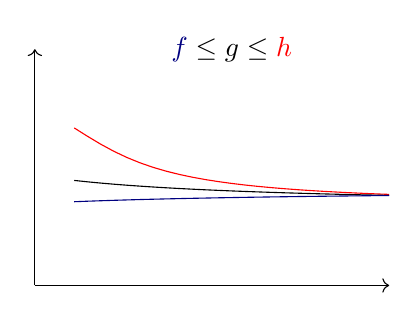
\begin{tikzpicture}
    		\draw[->] (-.5,0) -- (4,0);
    		\draw[->] (-.5,0) -- (-.5,3);
    		\draw[domain=0:4,variable=\x,red]  plot (\x,{2-atan(\x)/90});
    		\draw[domain=0:4,variable=\x]	     plot (\x,{1+1/(\x+3)});
    		\draw[domain=0:4,variable=\x,NavyBlue] plot (\x,{(1+1/(\x+3))^(\x+3)/2.23});
    		\node at (2,3) {$\textcolor{NavyBlue}{f} \leq g \leq \textcolor{red}{h}$};
    	\end{tikzpicture}
    \end{figure}

    \begin{theorem}\textbf{Squeeze Theorem}\\
        If $f(x)\leq g(x)\leq h(x)$, on $(a,b)$ 
        and $\dlim_{x\to a^+}f(x)=L=\dlim_{x\to a^+} h(x)$,
        then $\dlim_{x\to a^+}f(x) = L$.
    \end{theorem}
    \begin{proof}
        If $\epsilon>0$, 
        \begin{description}
            \item $\dlim_{x\to a^+} f(x)=L$, means that 
            $\exists\,\, \delta_1>0$, $a<x<a+\delta_1 \Rightarrow \abs{f(x)-L}<\epsilon$.
            \item $\dlim_{x\to a^+} g(x)=L$, means that 
            $\exists\,\, \delta_2>0$, $a<x<a+\delta_2 \Rightarrow \abs{h(x)-L}<\epsilon$.
        \end{description}
        so if $a<x<a+\min\{\delta_1, \delta_2\}$, 
        then $L-\epsilon<f(x)\leq g(x)\leq h(x)<L+\epsilon \Rightarrow \abs{g(x)-L}<\epsilon$
    \end{proof}

    {\color{Brown}
    \textbf{Example 1: $\dlim_{\theta \to 0} \frac{\sin \theta}{\theta}=1$}

    \textbf{Example 2:} 
        \begin{align*}
            \dlim_{\theta \to 0} \frac{1-\cos \theta}{\theta^2}
            &=\dlim_{\theta \top 0} \frac{(1-\cos \theta)
            (1+ \cos\theta)}{\theta^2(1+\cos\theta)}\\
            &=\dlim_{\theta \to 0} \frac{1-\cos^2 \theta}
            {\theta^2(1+\cos \theta)}\\
            &=\dlim_{\theta \to 0} \frac{\sin^2 \theta}
             {\theta ^2}\frac1{1+\cos \theta}\\
            &=\frac12\\
        \end{align*}}

    \begin{proposition}
        If $\dlim_{x\to a}f(x) = L$ and $
        \dlim_{x\to a}f(x) = M$, then 
        \begin{enumerate}
            \item $\dlim_{x\to a} c\cdot f(x) =c\cdot L$
            \item $\dlim_{x\to a} f(x) + g(x) = L+M$
            \begin{proof}
                Let $\epsilon>0$, use value $\epsilon / 2$
                
                There exists $N_1$ such that for all $n\geq N_1$,
                $\abs{f(x)-L}<\frac{\epsilon}2$;
                there exists $N_2$ such that for all $n\geq N_2$,
                $\abs{g(x)-M}<\frac{\epsilon}2$;

                Hence $\abs{f(x)+g(x) - L-M} \leq \abs{f(x)-L}+\abs{g(x)-M}
                <\frac{\epsilon} 2 + \frac{\epsilon} 2=\epsilon$
            \end{proof}
            \item $\dlim_{x\to a} f(x)g(x)=LM$
            \item $\dlim_{x\to a}$ if $M\neq 0$, 
            then $\exists \delta>0$, s.t. $g(x)\neq 0$,
            $(a-\delta, b+\delta) \backslash \{a\}$ and
                $\frac{f(x)}{g(x)} = \frac LM$
        \end{enumerate}

    \end{proposition}

    Problem: graph $\sin x / x $,  $x\sin \frac 1x$
    \vspace{1in}
    \subsection{The Natural Logarithm and $e$}
    For $0<a<b<\infty$, let $A(a,b)$ denote
    the area under $y=\frac1x$ from $x=a$ to $x=b$.
    
    If $0<b<a<\infty$, Let $A(a,b)=-A(a,b)$.

    Define $L(x) = A(1, x)$, then 
    \begin{itemize}
        \item $A(a,a)=0$
        \item $A(a,b)+A(b,c) = A(a,c)$
        \item if $s>0$, then $A(s_a, s_b)=A(a,b)$\\
    \end{itemize}

    \begin{proposition}
        If $a, b>0$, $L(a) + L(b)=L(ab)$.
    \end{proposition}
    \begin{proof}
        $L(a)+L(b)=A(1,a)+A(1,b)=A(1,a)+A(a,ab)=A(1,ab)=L(ab)$\\
    \end{proof}

    \begin{corollary}
        If $a>0$, $L(a^n) = nL(a)$ for $n \in \mathbb{Z}$.
    \end{corollary}
    \begin{proof}
        $n=0$, $L(a^0) = 0L(a)=A(1,1)=0=0L(a)$.
        
        If we have shown that $L(a^n) = nL(a)$, $n\geq 0$.
        then $L(a^{n+1})=L(a^n\cdot a)=L(a^n)+L(a) =nL(a)+L(a)=(n+1)L(a)$.

        By Induction, true for all $n \in \mathbb{N}$.

        $0=L(1)=L(a^n\cdot a^{-n})=L(a^n)+L(a^{-n})=nL(a)+L(a^{-n})
        \Rightarrow L(a^n)=nL(a)$\\
    \end{proof}

    \textbf{Remark:} $L(x)$ is strictly monotone increasing. 

    $\dlim_{x\to+\infty} L(x) = \dlim_{n\to+infty} L(2^n)
    =\dlim_{n\to+\infty} nL(2)=\infty$\\

    \begin{definition}
        There is a unique number $e$ such that $L(e) = 1$, $e\approx 2.71828\cdots$
    \end{definition}
    
        $L(2.5) < 1\frac{1+1/2}2+\frac12 \frac{0.5+2/3}2=\frac {37}{40}<1$
        
        $L(3)< A(1,2)+(A2,3) = \frac{16}{15}>1$

        $\therefore 2.5<e<3$


    \begin{proposition}
        $L$ is differentiable and $\frac d{dx} \,\, L(x) = \frac1x$
    \end{proposition}

    \begin{definition}\textbf{Natural Logarithm}
         The natrual logarithm $\ln x$ or $\log x$ is the function $L(x)$ defined.
        \begin{itemize}
            \item $\ln x$ is monotone increasing.
            \item $\ln a^n = n\ln a$
            \item $\ln 1 = 0$ \,\, and \,\, $\ln e = 1$
            \item $\dlim_{x\to\infty} \ln x = +\infty$
            \item $\dlim_{x\to 0^+} \ln x = 
            -\dlim_{x\to 0^+} \ln \frac1x = -\dlim_{y\to\infty} \ln y=-\infty$\\
        \end{itemize}
    \end{definition}

    \begin{figure}[htbp]
    	\centering
    	\caption{The area under the function $\frac1x$ is $\log x$}
    	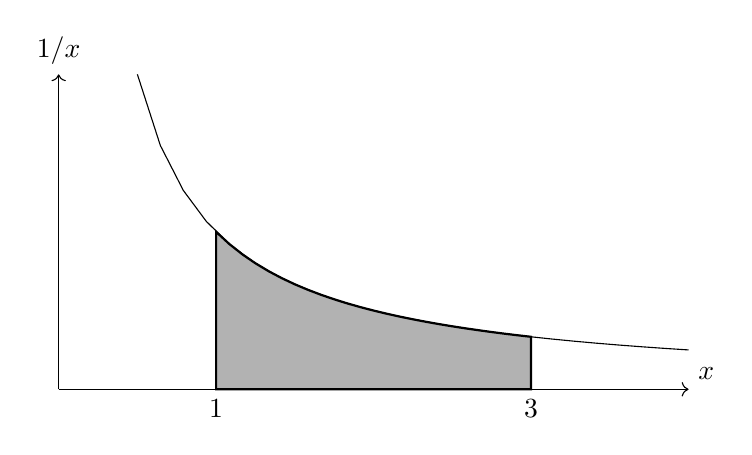
\begin{tikzpicture}[scale=2]
    		%\draw[domain=0.2:5,variable=\x] plot (\x,{ln(\x)});

    		\draw[->] (0,0) -- (0,2) node[above] {$1/x$};
    		\draw[->] (0,0) -- (4,0) node[above right] {$x$};

    		\draw[domain=0.5:4,variable=\x,black]
					plot (\x,{1/\x});
    		\filldraw[black!30,domain=1:3,variable=\x,draw=black,thick]
					(1,0) node[below,black,opacity=1] {$1$}
					-- plot (\x,{1/\x}) -- (3,0) node[below,black,opacity=1] {$3$}
					-- cycle;
    	\end{tikzpicture}
    \end{figure}

    {\color{Brown}
    \textbf{Example 1: $\dlim_{x\to\infty} \frac{\ln x}x=0$}
    \begin{proof}
        Since $2^n\to\infty$.  Let $a_n = \dfrac{\ln x^n}{2^n}=
        \dfrac{n\ln2}{2^n}$

        If $n\geq 2$, then $\dfrac{a_{n+1}}{a_n}=\dfrac{(n+1)\ln 2}{2^{n+1}}
        \cdot \dfrac{2^n}{n\ln 2}
        =\dfrac{n+1}{2n}=\dfrac12+\dfrac1{2n}\leq \dfrac34$.

        $0\leq a_{2+k}\leq \dfrac34 \cdot a_{2+k-1}
        \leq\cdots\leq (\dfrac34)^k\cdot a_2$, $\abs{\dfrac34}<1$,
        so $(\dfrac34)^n\to 0$.

        If $x^n\leq x\leq 2^{n+1}$, then $\ln 2^n\leq \ln x\leq \ln 2^{n+1}$,
        
        $\therefore\quad \dfrac{n\ln 2}{2^{n+1}}\leq \dfrac{\ln x}x \leq (\dfrac{(n+1)\ln2}{2^{n+1}})2$.

        By Squeeze Theorem, $\dlim_{x\to\infty} \frac{\ln x}x =0$.\\
    \end{proof}

    \textbf{Example 2:} If $a>0$, $\dlim_{x\to\infty} \frac{\ln x}{x^a}=
    \dlim_{y\to\infty} \frac{\ln y^{\frac1a}}y 
    =\frac1a \cdot \dlim_{x\to\infty} \frac{\ln y} y =0$\\

    \textbf{Example 3:} $\dlim_{x\to 0^+} x^a \ln x 
    = \dlim_{y\to\infty} y^{-a}\ln \frac 1y
    = \dlim_{y\to\infty} \frac{-\ln y}{y^a} =0$}\\


    \begin{definition}\textbf{Inverse Function}
        If $f:x \to y$ is $1:1$, $Ran(f): Z\leq y$, 
        then there is an inverse function
        $f^{-1}:Z \to y$, s.t. $f(x)=Z$ $\iff $ $f^{-1}(Z)=x$. \\
    \end{definition}

    \begin{definition}
        The inverse of $\ln x$, in $(0, \infty) \to (-\infty, +\infty)$ 
        is the exponential function $f(x) = e^x$.

        $f(x) = e^x: (-\infty, +\infty) \to (0, \infty)$.\\
    \end{definition}

    {\color{Brown}\textbf{Example 1: $\dlim_{x\to+\infty} \frac{e^x} {x^a}$}

    Let $x=\ln y$, then $\dlim_{x\to+\infty} \frac{e^x} {x^a} 
    = \dlim_{y\to+\infty} \frac{e^{\ln y}}{(\ln y)^a} 
    =\dlim_{y\to\infty} \frac y{(\ln y)^n}=+\infty$}\\

    \begin{proposition}
        $\frac d{dx} e^x = e^x$
    \end{proposition}
    \begin{proof}
        \begin{align*}
            \ln (e^x) &= x\\
            \frac1{e^x} \cdot \frac{d}{dx} e^x &= 1\\
            \therefore\,\, \frac d{dx} e^x&=e^x
        \end{align*}
    \end{proof}

    \textbf{Remark:} 
    \begin{description}
        \item $\dlim_{x\to+\infty} e^{\frac1x}x =\infty$
        \item $\dlim_{x\to -\infty} e^{\frac 1x}x =-\infty$
        \item $\dlim_{x\to+\infty} e^{\frac1x} x-x 
            =\dlim_{x\to+\infty} x(e^{\frac1x }-1) 
            =\dlim_{y\to 0^+} \frac{e^y -1} y =1$
    \end{description}

    \begin{proposition}
        $\dlim_{n\to\infty} (1+\frac xn)^n = e^x$ \qquad $e$ is monotone 
        increasing
    \end{proposition}

    \begin{proof}
        Case 1: $x\geq 0$, 
        \begin{align*}
            \frac xn \cdot \frac1{1+\frac xn}&<\ln (1+\frac xn)
            <1 \cdot \frac xn \\ 
            \frac{x}{1+\frac xn}&<n \ln (1+\frac xn)<x\\
            \therefore \exp \frac{x}{1+\frac xn}&<\exp (n\ln 1+\frac xn)<e^x\\
            e^x&<(1+\frac xn)^n < e^x
        \end{align*}
        \begin{center}
            $\therefore\,\, \dlim_{n\to\infty} (1+\frac xn)^n = e^n$ when $x\geq 0$
        \end{center}
        Case 2: $x< 0$, let $h = \frac{-x}n$, $0<h<1$, 
        \begin{align*}
            1\cdot h &\leq A(1-h, 1)\leq \frac1{1-h} + h\\
            %
            1&\leq \frac{\ln (1-h)}{-h}=\frac{-A(1-h,1)}{-h}\leq \frac 1{1-h}\\
            %
            1&\leq \frac{\ln (1+\frac xn)}{\frac xn}\leq \frac1{1+\frac xn}\\
            %
            x&\geq n\ln(1+\frac xn)\geq \frac x{1+\frac xn}\\
            %
            e^x&\geq (1+\frac xn)^n \geq \exp\frac x{1+\frac xn}
        \end{align*}
        \begin{center}
            $\therefore\,\, \dlim_{n\to\infty} (1+\frac xn)^n = e^n$ when $x<0$.
         \end{center}
         
        Hence $\dlim_{n\to\infty} (1+\frac xn)^n = e^x$.
    \end{proof}

    \vspace{1.5 in}

    \newpage
    \subsection{Continuity}
    \begin{definition}
        $f(a,b) \to\mathbb{R}$, $a<c<b$, then $f$ is continuous at $c$
        if $\dlim_{x\to c} f(x) =f(c)$.

        $(x-\delta version) \forall \epsilon>0$, $\exists \delta >0$ s.t. 
        $\abs{x-c}<\delta \to \abs{f(x)-f(c)}<\epsilon$.
        
        If $f:(a,b)\to\mathbb{R}$ say is continuous at $a$
        if $\dlim_{x\to a^+} f(x) = f(a)$; and continuous at
        $b$ if $\dlim_{x\to b^-}f(x) =f(b)$.

        Say $f$ is continuous on a set $A$ if $f$ continuous at every $a\in A$.\\
    \end{definition}

    {\color{Brown}
    \textbf{Example 1:
    	$f(x)=\frac 1x$, for $x\neq 0$, $a\neq 0$, given $\epsilon > 0$,
        estimate $\abs{f(x)-f(a)}$.}

    Want $\delta >0$, s.t. $\abs{x-a}<\delta \Rightarrow \abs{f(x)-f(a)}<\epsilon$.
    
    Set $\epsilon_1 = \frac{\abs{a}}{2}$. If $\abs{x-a}<\frac{\abs a}2$, then
    $\abs{x} =\abs{x-a+a}\geq \abs a-\abs{x-a}> \abs{a}-\frac{\abs a}2 =\frac{\abs a}2$.

    Let $\delta_2 = \frac{\epsilon \abs{a}^2}{2}$, $\therefore 
    \delta = \min \{\frac{\abs a}2, \frac{\epsilon \abs{a}^2}2\}$,
  
    then $\abs{f(x)-f(a)}=\abs{\frac1x -\frac1a}
    =\abs{\frac{a-x}{ax}}\leq \frac{\abs{a-x}}{\abs a\cdot \frac{\abs a}2}
    =\frac{2\abs{a-x}}{\abs{a}^2}
    <\frac{2}{\abs a^2}\cdot \frac{\epsilon\abs{a}^2}{2}=\epsilon$\\


    \textbf{Example 2:
    $f(x) =\sin x$, let $x=a+h$, estimate $\abs{f(x)-f(a)}$.}

    Since $\abs{x-a}<\delta \iff \abs h< \delta$.

    Let $\epsilon > 0$, 
    $\sin (a+h)=\sin a \cos h+\sin h\cos a$. 

    $\abs{\sin (a+h)-\sin a}\leq \abs{\sin a(\cos h-1)}
    +\abs{\cos a\cdot \sin h}$.

    Showed:
    \begin{description}
        \item  $h\in [0,\frac{\pi}2]$, $1-h^2\leq \cos h\leq 1$ \quad and \quad
            $0<\sin h<h$. 
        \item  $h\in[-\frac{\pi}2, \frac{\pi}2]$, $-h^2\leq \cos h-1\leq 0$ 
        \quad and \quad $h<\sin h<0$.
    \end{description}

    If $\abs h<1$, 
    $\abs{\sin (a+h)-\sin a}\leq \abs{\sin a(\cos h-1)}
    +\abs{\cos a\cdot \sin h}\leq 1\cdot h^2 +1\cdot\abs{h}\leq 2\abs{h}$.

    Take $\delta = \min \{\frac{\epsilon}2, 1\}$.

    Hence, $\abs{\sin (a+h)-\sin a}\leq 2\abs{h}<2\delta\leq \epsilon$.\\


    \textbf{Example 3: 
        $f(x) =\cos x=\sin (-x +\frac{\pi}2)$} is continuous. \\


    \textbf{Example 4: 
        $f(x) = \ln x$, $x>0$, $\abs{x-a}<\delta$.}

    Let $\delta = \min \{\frac {a\epsilon}2, \,\,\frac a2\}$, 
    $\abs{f(x)-f(a)}=$ $\abs{A(x,a)}
    \leq $ $\abs{x-a} \cdot \max\{\frac 1a,\,\, \frac 1x\}
    <\,\,\frac 2a\, \abs{\,x-a}$.\\


    \textbf{Example 5: $f(x) = 
        \begin{cases}
            \dfrac{\sin x}x, &x\neq 0\\
            1 , &x=0\\
        \end{cases}$}

    $\dlim_{x\to 0} \frac {\sin x} x = 1 = f(0)$ \qquad
    $\therefore$ continuous.\\

    \textbf{Example 6: $f(x)=
        \begin{cases}
            1, &x>0\\
            0, &x=0\\
            -1, &x<0\\
        \end{cases}$}

    $\dlim_{x\to 0^+} f(x)=1\neq \dlim_{x\to 0^-} f(x) = -1$ \qquad
    $\therefore$ not continuous.\\

    \textbf{Example 7: $f(x)= 
        \begin{cases}
            x, &x\in \mathbb{Q}\\
            0, &x\in \mathbb{R\backslash Q}\\
        \end{cases}$}

	continuous at $x=0$, discontinuous at every $x\neq 0$.\\

    \textbf{Example 8: $f(x) = \begin{cases}
        0, &x\in \mathbb{R}\backslash \mathbb{Q}\\
        \frac 1q, &\text{if } x=\frac pq, 
        \,q>0, \,\gcd (p,q)=1, \,\,p,q \in \mathbb{Z}\\
    \end{cases}$}

    $x\in\mathbb{Q}$, $\forall \delta >0$, $\exists y \not\in \mathbb{Q}$,
    $\abs{x-y}<\delta$. not continuous.

    $x\in\mathbb{R}$, $\epsilon > 0$, 
    $\exists \frac 1N < \epsilon$ , if $0<\abs x<\frac1N$, 
    $x \not\in \mathbb{Q}$, or $x\neq \frac pq$, $q\geq N$,

    so $\abs{x}\leq \frac 1N<\epsilon$. $\dlim_{x\to 0} f(x) \neq 0$.
    
    $f(x)$ is continuous on $\mathbb{R}\backslash \mathbb{Q}$, 
    discontinuous on $\mathbb{Q}$.\\
    


  \textbf{Example 9: $f(x) = \sin \frac 1x$, $x\neq 0$, continuous.}}\\\\

    \begin{proposition}
        If $f, g$ are functions on $(a,b)$, which are continuous at $c$, 
        $a<c<b$, then
        \begin{enumerate}
            \item $\alpha f(x)$ is continuous,
            \item $f(x)+g(x)$ is continuous,
            \item $f(x)g(x)$ is continuous,
            \item $g(x)\neq 0, 
            	\frac{f(x)}{g(x)}$ is continuous at $x$ if $x\neq 0$,
            \item $p(x) = a_0+a_1x+a_2x^2+a_3x^3+a_4x^4+\cdots+a_nx^n$
            	is continuous.\\
        \end{enumerate}
    \end{proposition}


\newpage
	\subsection{Composite Functions}
    \begin{definition}{\textbf{Composition of Functions}}\\
    $(g\cdot f)(x)=g(f(x))$, $\Img f \subseteq \Dom  g$\\
    \end{definition}

    \begin{proposition}
        If $\Img f \subseteq \Dom g$, $\dlim_{x\to a} f(x) = b$, 
        then $\dlim_{y\to b}g(y) = c = g(b)$, then $\dlim_{x\to a} g(f(x))=c$.
        
        In particular, if $f$ is continuous at $a$ and $g$ is continuous at $f(a)$,
        then $g \circ f$ is continuous at $a$.
    \end{proposition}

    \begin{proof}
        Let $\epsilon > 0$, since $\lim_{y\to b} g(y)=c$, $\exists \delta >0$,
        s,t, $0\leq \abs{y-b}<\delta \Rightarrow\abs{g(y)-c}<\epsilon$.

        Since $\lim_{x\to a} f(x) = b$, using $\delta > 0$, $\exists \delta > 0$,
        s.t. 
        \begin{align*}
            0<\abs{x-a}&<\delta\\
            \abs{f(x)-b}&<\delta\\
            \abs{g(f(x))-c}&<\epsilon
        \end{align*}
        In particular, if $f$ continuous at $a$, then $b=f(a)$, $c=g(b)=g(f(a))$,
        and $\lim_{x\to a} g(f(x))=c=g(f(a))$, so $g\circ f$ is continuous at $a$.\\
    \end{proof}

    \begin{proposition}
        If $f(x)$ and $g(x)$ are continuous, 
        $\Img f \subseteq \Dom g$, then $g \circ f$ is continuous.\\
    \end{proposition}

		\begin{theorem}
    	If $f(x)$ is continuous then $\abs{f(x)}$ is continuous.
    \end{theorem}
		\begin{proof}
			Since $f(x)$ is continuous, therefore, when $x_n\to x_0$, 
			\[
				\abs{\abs{f(x_n)}-\abs{f(x_0)}} \leq \abs{f(x_n)-f(x_0)}\to 0
			\]
			Therefore, $\abs{\abs{f(x_n)}-\abs{f(x_0)}}\to 0$, hence $\abs{f(x)}$ is 
			continuous.
		\end{proof}
    \begin{theorem}[\textbf{Bolzano's Theorem}]
			Let $f$ be a continuous function on $[a,b]$ with $f(a)f(b)<0$, then there
			is at least one $c\in(a,b)$ for which $f(c)=0$.
    \end{theorem}
    \begin{proof}
    	The proof can be done with IVT.
    \end{proof}


\newpage
	\subsection{EVT and IVT}
    {\color{Blue}
	 \begin{theorem}{\textbf{Extreme Value Theorem}}
        $f:[a,b]\to \mathbb{R}$ is continuous, 
        then $f$ attains its $\min$, $\max$ values.
    
        i.e. $\exists x_1, x_1\in [a,b], s.t. f(x_1)=\sup f(x)$ and 
        $f(x_2) = \inf f(x)$.
    \end{theorem}
    \begin{proof}
        Let $L =\sup f(x)$, $a\leq x\leq b$, (possibly $+\infty$).

        Choose $L_1<L_2<L_3<L_n<L_{n+1}\cdots$ s.t. $\lim_{n\to\infty} L_n=L$. 

        If $L<\infty$, let $L_n=L-\frac 1n$. If $L=+\infty$, let $L_n=n$.

        $L_n<\sup f(x)$, so we can pick $x_n \in [a, b]$ such that 
        $f(x_n) > L_n$, 
        and $(x_n)_{n=1}^{+\infty}$ is a bounded sequence.

        By the Bolzano-Weierstrass Theorem, there is a subsequence 
        $x_{n_1}$, $x_{n_2}$,$x_{n_3}$, $\cdots$ s.t. 
        $\lim_{i\to\infty} x_{n_i}=x_0$ exists.

        $a\leq x_{n_i}\leq b$, so $a\leq x_0\leq b$. 
         
        Since $f$ is continuous,
        $\sup f(x)= L\geq f(x_0)=\dlim_{i\to\infty} f(x_{n_i})\geq
        \dlim_{n\to\infty}L_n=L$.

        $f(x_0) = L = \sup f(x)<\infty$ because $f(x_0)\in\mathbb{R}$.

        For the minimum, either repeat proof using $M=\inf f(x)$ 
        or find the $\max$ of $-f(x)$. 
        
    \end{proof}}

    {\color{Brown}
    \textbf{Example 1: $f(x) =1 -\abs x$ on $[-2,2]$}
    \begin{itemize}
        \item $f(0) = 1 = \sup f(x)$
        \item $f(-2) = -1 = f(2) = \inf f(x)$\\
    \end{itemize}

    \textbf{Example 2: $f(x)=\frac 1{1+x^2}$, $f:(-\infty, \infty)$}
    \begin{itemize}
        \item $\sup f(x) = 1$
        \item $\inf f(x) = 0$ not attained \\
    \end{itemize}

    \textbf{Example 3: $f:(0, 1) \to \mathbb{R}$, $f(x) = \cot \pi x$}
    \begin{itemize}
        \item $\sup f(x) = +\infty $
        \item $\inf f(x) = +\infty $\\
    \end{itemize}

    \textbf{Example 4: $f: [0,1]$, $f(x) = \begin{cases}
        x, &0<x<1\\
        \frac 12, & x=0 \quad or \quad x=1
    \end{cases}$}

    $f$ is not continuous and the theorem does not apply.}\\\\


	\newpage
    \begin{theorem}{\textbf{Intermediate Value Theorem}}
        Let $f: [a,b] \to \mathbb{R}$ be a continuous function.

        Suppose that $f(a)<L<f(b)$ or $f(a)>L>f(b)$, then there is a point $c$, 
        $a<c<b$ s.t. $f(c) = L$.
    \end{theorem}
    \begin{proof}
        Let $x =\{x \in [a,b]: f(x)<L\}$.

        Assume $f(a)< L<f(b)$, then $a\in X$, $b\not\in X$,
        By LUBP, $c =\sup X$ exists.

        Claim $a<c<b$, 
        
        $f$ is continuous at $a$, 
        so let $\epsilon =L-f(a)>0$, 
        there is a $\delta_1>0$, $a\leq x<a+\delta_1 
        \Rightarrow f(x)<f(a)+\epsilon =L$,
        so $[a, a+\delta_1) \subseteq X$. 

        $f$ is continuous at $b$, 
        so let $\epsilon =L-f(b)>0$, 
        there is a $\delta_2>0$, $b-\delta_2< x\leq b
        \Rightarrow f(x)<f(a)-\epsilon =L$,
        so $(b-\delta_2, b]$ is disjoint from $X$.
        
        $a+ \delta _1\leq c\leq b-\delta_2$, 

        Find $x_n\in X$, $c-\frac1n<x_n\leq c$, so $x_n\to c$.
        
        $f$ is continuous, $f(c)=\lim_{n\to\infty} f(x_n)\leq L$,
        if $x>c$, $f(x)\geq L$, (not in $X$). 

        $\lim_{n\to\infty} y_n =c$, $f(y_n)\geq L$,
         $f(c) = \lim_{n\to\infty} f(y_n)\geq L$.

         $\therefore f(c)=L$.\\
    \end{proof}


	 {\color{Brown}
    \textbf{Example 1: Every polynomial $P(x)$ of degree $P\geq 1$ with odd 
    degree has a real root.}

    $P(x) = a_{2n+1} x^{2n+1} + a_{2n}x^{2n}+\cdots+a_1 x+a_0$, 
    $a_{2n+1}\neq 0$. 
    \begin{align*}
        \dlim_{x\to\infty} P(x)
        &=\dlim_{x\to+\infty} a_{2n+1}x^{2n+1} 
        (1+ \frac{a_{2n}}x + \cdots + \frac{a_0}{x^{2n+1}})\\
        &=\begin{cases}
            +\infty, \text{if } a_{2n+1}>0 \\
            -\infty, \text{if } a_{2n+1}<0
        \end{cases}\\
        \dlim_{x\to-\infty} P(x)
        &=\begin{cases}
            -\infty, \text{if } a_{2n+1}>0 \\
            +\infty, \text{if } a_{2n+1}<0
        \end{cases}
    \end{align*}
    Say $a_{2n+1}>0$, \begin{description}
        \item $\exists x_1$ s.t. $P(x_1)>157$,
        \item $\exists x_2$ s.t. $P(x_2)<-341$, 
    \end{description}

    By IVT, $\exists c\in (x_2, x_1)$ s.t. $P(c)=0$.}\\


    \begin{corollary}{\textbf{for IVT}\\}
        If $f: [a, b] \to \mathbb{R}$ is continuous, 
        then $\Img f = f([a,b])$ is a closed bounded interval.
    \end{corollary}
    \begin{proof}
        By EVT, $\exists x_1, x_2 \in [a,b]$,

        $f(x_1)=d =\sup f(x)$, $f(x_2)=c =\inf f(x)$

        If $c\leq L<d$, by $I.V.T$, $\exists x$ s.t. $f(x)=L$.

        $\therefore f([a,b])= [c,d]$.
    \end{proof}

    \vspace{1.0 in }
    
    \subsection{Monotone Functions}
    \begin{definition}[\textbf{Monotone}]
		A function $f$ is called increasing on an interval $(a,b)$ if 
		$f(x)\leq f(y)$ where $a<x\leq y<b$. 
		
		It is strictly increasing on $(a,b)$
		if $f(x)<f(y)$ whenever $a<x\leq y<b$. 

		Similarly, we define decreasing and strictly decreasing function. 
		All of these functions are called monotone. 
	\end{definition}

    \begin{proposition}
        Let $f:(a,b)\to\mathbb{R}$ be monotone increasing (decreasing). 
        
        If $a<b<c$, then $\dlim_{x\to c^-}f(x) =L$ exists, 
        and $\dlim_{x\to c^+}f(x) =M$ exists.
        
        $L \leq f(x) \leq M$ (or $L\geq f(c)\geq M)$\\
    \end{proposition}

    \begin{definition}
        If $\dlim_{x\to c^-}f(x) =L$, and $dlim_{x\to c^+}f(x) =M$,
        and $L\neq M$, this is called a \textbf{jump discontinuity.}\\
    \end{definition}

    \begin{corollary}
        The only discontinuities that a monotone function can have
        are jump discontinuities.\\
    \end{corollary}
 
    \begin{corollary}
        If $f:(a,b) : \mathbb{R}$ is monotone, then $f$ is continuous
        $\Leftrightarrow$ $\Img f$ is an interval.
    \end{corollary}
    \begin{proof}
        If $f$ is continuous, then $\Img f$ is an interval by 
        IVT. 

        If $f$ is discontinuous, then it has a jump discontinuity,
        say at $x=c$, $dlim_{x\to c^-}f(x) =L<Mdlim_{x\to c^+}f(x)$.
        
        The $\Img f \subseteq (\dlim_{x\to a^+} f(x), L)
        \cup \{f(c)\}\cup(M,\dlim_{x\to a^-} f(x))$\\ 
    \end{proof}

    \begin{corollary}
        Let $f:(a,b) : \mathbb{R}$ bet strictly monotone increasing(decreasing)
        and continuous,
        with $\Img f = (c , d)$. 
        Then, the inverse function $f^{-1}:(c,d) \to (a,b)$ is also continuous.
    \end{corollary}

    \begin{proof}
        If $f(x)<f(y)$, so $f$ is $1-1$. $f$ is continuous, 
        so $\Img f$ is an interval.

        So $f^{-1}:(c, d)\to (a,b)$ is defined by $f^{-1} (x)$ if $f(x) = y$.
        Since $\Img f^{-1}$ is an interval, $f^{-1}$ is continuous by Cor 3.6.2.

        If $f(x_1) = y_1$, $f(x_2) < y_2$ $\Rightarrow$ $x_1<x_2$,        
        so $y_1<y_2 \Rightarrow f^{-1}(y_1)<x_1<x_2=f^{-1}(y_2)$.
        
        Therefore, $f^{-1}$ is strictly monotone incresing(decreasing).\\
    \end{proof} 

    {\color{Brown} 
    \textbf{Example 1: }
    
    $\sec : [0, \frac{\pi}2) \to [1, -\infty),
    (\frac{\pi}2, \pi] \to (-\infty, 1]$.
     
    $\sec^{-1} : [1, \infty) \to [0, \frac{\pi}2), 
    (-\infty, -1] \to (\frac{\pi}2, \pi]$\\


    \textbf{Example 2: Cantor Ternary Function (continuous)}}

%    $C(x): $ \begin{description}
%        \item $[\frac13, \frac23]$
%    \end{description}

    \newpage
    \subsection{Cardinality and Countable Sets}
    \begin{definition}
        Say two sets $A$ and $B$ have the same cardinality.

        If $\exists f: A \to B$ which is $1-1$ and onto, 
        write $\abs{A} = \abs{B}$.

        Say $\abs{A}\leq \abs{B}$, if $\exists f: A \to B$ which is $1-1$,
        then $A$ is countable if $\abs{A} = \mathbb{\mathbb{N}}$.\\
    \end{definition}

    {\color{Brown}
    \textbf{Example 1: }

    $2\mathbb{N} = \{2, 4, 6, 8, \cdots\}$    
    $\abs{2\mathbb{N}}=\abs{N}$
     
    $f:2\mathbb{N} \to \mathbb{N}$, $f(2n)=n$\\

    \textbf{Example 2:}

    $\mathbb{Z} = \{0 ,1, -1, 2, -2, \cdots\}$ \qquad 
    $\abs{\mathbb{Z}}=\abs{\mathbb{N}}$ 

    $f(b) = 
        \begin{cases}
            2n+1,    & n\leq 0\\
            2\abs{n}, & n<0\\
        \end{cases}$\\

        \textbf{Example 3: $\mathbb{N} \times \mathbb{N} = 
    \{(m,n), \,\,m,n\in\mathbb{N}\}$ }\\

    \textbf{Example 4: $\mathbb{Q} = \{\frac pq,
    q\in\mathbb{N}, p \in \mathbb{Z}\}, \gcd(p,q)=1$.}

    $f: \mathbb{Q} \to \mathbb{Z} \times\mathbb{N}$,
    \qquad $\abs{\mathbb{Q}}\leq \abs{\mathbb{Z}\times\mathbb{N}}
    \leq\abs{\mathbb{Z}}=\abs{\mathbb{N}}$}\\
    

    \begin{proposition}
        If $A$ is an infinite set, and $\abs{A}\leq \abs{\mathbb{N}}$,
        then $\abs{A} = \abs{\mathbb{N}}$.
    \end{proposition}
    \begin{proof}
        Let $f:A\to\mathbb{N}$ be $1-1$, then $\abs{A}=\mathbb{N}$, 
    \end{proof}

    \newpage
\section{Differentiation}
    \subsection{Basics}
    \begin{definition}
        $f:(a,b)\to\mathbb{R}$, say  $f$ is differentiable at $x$ 
        if $\dim_{h\to 0} \frac{f(x+h)-f(x)}h$ exists. The limit is $f'(x)$
        or $\frac d{dx} f(x)$. 

        Say $f$ is differentiable on $(a,b)$, if it is differentiable at $x$,
         for every $x\in (a,b)$.\\
    \end{definition}
     
		\begin{definition}
			The tangent line to $f$ at $x$ is 
			\begin{center}
				$T(x+h) = f(x)+f'(x)h$\\
				$T(y) = f(x) + f'(x) (y-x)$
			\end{center}
		\end{definition}

    This is the best linear approximation near $x$. 
    Line through $(x, f(x))$ with slope $f'(x)$.\\

    \begin{theorem}
        If $f$ is differentiable of $x=c$, 
        then $f$ is continuous at $x=c$.
    \end{theorem}
     \begin{proof}
        \begin{align*}
				 \dlim_{x\to c} f(x)- f(c) 
					&= \dlim_{x\to c} \frac{f(x)-f(c)}{x-c}\cdot (x-c)\\
					&=\dlim_{x\to c} \frac{f(x)-f(c)}{x-c} \dlim_{x\to c}(x-c)\\
					&=\dlim_{h\to 0} \frac{f(c+h)-f(c)}h \cdot \dlim_{x\to c}(x-c)\\
					&=f'(c)\cdot 0 = 0
        \end{align*}
        $\therefore \dlim_{x\to c} f(x) = f(c)$ so $f$ is continuous at $c$. \\
    \end{proof}

    
    \begin{proposition}
        Let $f:(a,b)\to\mathbb{R}$, $x_0\in(a,b)$, TFAE:
        \begin{enumerate}
					  \item $f$ is differentiable at $x_0$, $f'(x_0) = m$
            \item let $T(x) = f(x_0) +f'(x_0)(x-x_0)$, 
            then $\dlim_{h\to 0} \frac{f(x_0+h)-T(x-x_0)}h = 0$
            \item $f(x) = T(x) + e(x)$ ($e$ stand for error), 
             $\dlim_{h\to 0} \frac{e(x_0+h)} h = 0$. (the difference
             from the line is small relative to $h = x - x_0$)
        \end{enumerate}
    \end{proposition}
    \begin{proof} Proving equivalent means proving they imply each other.

        From 1 to 2: $\dlim_{h\to 0} \frac{f(x_0+h)-f(x_0)}h = m$.
				\begin{align*}
				\dlim_{h\to 0}\frac{f(x_0+h)-T(x_0+h)}h 
        &=\lim_{h\to 0} \frac{f(x_0+h) -f(x_0) -mh} h \\
        &= \dlim_{h\to 0} \frac{f(x_0+h)-f(x_0)}h - m = 0
				\end{align*}
       
        From 2 to 3: Define $e(x) = f(x) - T(x)$. 
        \[
        	\dlim_{h\to 0} \frac{e(x_0+h)}h 
					=\dlim_{h\to 0} \frac{f(x_0+h)-T(x_0+h)}h = 0
				\]

        From 3 to 1: $f(x) = T(x) + e(x) = f(x_0)+m(x-x_0)+e(x)$
         and $\dlim_{h\to 0} \frac{e(x_0+h)} h = 0$,
         \[
         	 \dlim_{h\to 0} \frac{f(x_0+h)-f(x_0)}h
						=\dlim_{h\to 0} \frac{f(x_0)+mh+e(x_0+h)-f(x_0)} h
						=\dlim_{h\to 0} m+\frac{e(x_0+h)}h = m
					\]

         $\therefore f'(x_0) = m$ and $f$ is differentiable at $x_0$.

    \end{proof}
    {\color{Brown}
    \textbf{Example 1: $f(x) = x^n$}
    \begin{align*}
        \dlim_{x\to 0} \frac{f(x+h) - f(x)}h 
        &=\dlim_{x\to 0} \frac{(x+h)^n-x^n}h \\
        &=\dlim_{x\to 0} \frac{x^n + \binom{n}{1} \cdot x^{n-1}h 
        + \binom{n}{2} \cdot x^{n-2} h^2 \cdots + \binom{n}{n} 
      \cdot h^n-x^n}h \\
        &= n x^{n-1}
    \end{align*}

    \textbf{Example 2: $f(x) = e^x$,}
    \begin{align*}
        \dlim_{h\to 0} \frac{e^{x+h}-e^x}{h}
        &=\dlim_{h\to 0} \frac{e^x(e^h-1)}h
        =e^x\dlim_{h\to 0} \frac{e^h-1}h
    \end{align*}
    Let $u = e^h$, $h\to 0 \iff u \to 1$
    \begin{align*}
        e^x\dlim_{h\to 0} \frac{e^h-1}h
        &=e^x\dlim_{u\to 1} \frac{u-1}{\ln u}\\
        &=\frac{e^x}{\dlim_{u\to 1} \frac{\ln u -\ln 1}{u-1}}\\
        &=\frac{e^x}{\dlim_{k\to 0} \frac{\ln (1+k)-\ln 1}k}
        =e^x
    \end{align*}

    \textbf{Example 3: }
    $f(x) = \begin{cases}
        x^2\sin \frac 1x, &x\neq 0\\
        0, &x=0
    \end{cases}$\\

    $f'(x) = 2x\sin\frac1x + x^2\cos \frac 1x \cdot -\frac1{x^2}
    =2x\sin\frac1x +\cos \frac 1x$

    $x=0$, \[
    	\dlim_{h\to 0} \frac{f'(h) - f(0)}h 
				= \dlim_{h\to 0} \frac{h^2\sin \frac1h}h 
				= \dlim_{h\to 0} h\sin \frac 1h
			\]

    $f$ is differentiable everywhere but is not continuous at 0.\\
 
    Remark: as $x\to \infty$, $x^2\sin \frac1x \approx x^2\frac 1x = x$
    \begin{align*}
        \dlim_{x\to \infty} x-f(x) 
        &= \dlim_{x\to\infty} x-x^2\sin \frac 1x\\
        &= \dlim_{u\to 0^+} \frac{1}u -\frac{\sin u}{u^2} \\
        &= \dlim_{u\to 0^+} \frac{u-\sin u}{u^2} \\
        &=\dlim_{u\to 0^+} \frac{1-\frac{\sin u}u}u \\
        &=0
  \end{align*}}

     \begin{proposition}
     	If $f$, $g$ are differentiable at $x_0$, then 
     	\begin{enumerate}
     	 	\item $(cf)'(x_0) = cf'(x_0)$

     	 	\item $(f+g)'(x_0)= f'(x_0)+g'(x_0)$

     	 	\item product rule  $(fg)'(x_0) = f(x_0)g'(x_0)+f'(x_0)g(x_0)$

     	 	\item quotient rule if $g(x_0) \neq 0$,
     	 		$(\frac fg)'(x_0) =\frac{f'(x_0) g(x_0) -f(x_0) g'(x_0)}{g(x_0)^2}$
     	 		
     	\end{enumerate}
    \end{proposition}
    \begin{proof}
        \begin{align*}
            (fg)'(x_0) &= \dlim_{h\to 0} \frac{f(x_0+h)g(x_0+h) -f(x_0) g(x_0)}{h}\\
            &=\dlim_{h\to 0} \frac{f(x_0+h)f(x_0+h)-f(x_0)g(x_0+h)
            +f(x_0)g(x_0+h)-f(x_0)g(x_0)}{h}\\
            &=\dlim_{h\to 0} \frac{f(x_0+h)-f(x_0)}h \dlim_{h\to 0}g(x_0+h)+
            f(x_0) \dlim_{x\to 0} \frac{g(x_0+h)-g(x_0)}h\\
            &=f'(x_0)\cdot g(x_0) + f(x_0)\cdot g'(x_0)
        \end{align*}
        \begin{align*}
            (\frac fg)'(x_0) 
            &=\dlim_{h\to 0} \frac{\frac{f'(x_0+h)}g(x_0+h)-\frac{f'(x_0)}{g'(x_0)}}h\\
            &=\dlim_{h\to 0} \frac{f(x_0+h)g(x_0)-f(x_0)g(x_0+h)}{hg(x_0+h)g(x_0)}\\
            &=\dlim_{h\to 0} \frac{f(x_0+h)g(x_0)-f(x0_0)g(x_0)+f(x_0)g(x_0)-f(x_0) g(x_0+h)}
            {hg(x_0+h) g(x_0)}\\
            &=\dlim_{h\to 0} \frac{f(x_0)+h-f(x_0)}h \frac{g(x_0)}{g(x_0+h)g(x_0)}
            -\frac{f(x_0)}{g(x_0+h)g(x_0)} \frac{g(x_0+h)-g(x_0)}h \\
            &=(\frac fg)'(x_0) =\frac{f'(x_0) g(x_0) -f(x_0) g'(x_0)}{g(x_0)^2}
        \end{align*}
    \end{proof}
    \newpage
    \begin{proposition} TFAE
        \begin{enumerate}
            \item $f$ is differentiable at $x_0$\\
            \item $f(x) =f(x_0) +\phi (x)(x-x_0)$ and $\phi$ is continuous at $x_0$\\
            \item In this case, $\phi(x_0) = f'(x_0)$
        \end{enumerate}
    \end{proposition}
    \begin{proof} 
        1 to 4: $\phi(x) =\begin{cases}
            \frac{f(x) -f(x_0)}{x-x_0}
            f'(x_0) 
        \end{cases}$ if $x\neq x_0$, 

        $\dlim_{x\to x_0} \phi(x) = \dlim_{x\to x_0} \frac{f(x)-f(x_0)}{x-x_0}
        =f'(x_0) =\phi(x_0)$

        4 to 1: 
        \begin{align*}
            f'(x_0)&=\dlim_{h\to 0} \frac{f(x_0+h) -f(x_0)}h\\
            &=\dlim_{h\to 0} \frac{f(x_0)+\phi(x_0+h)-f(x_0)}h \\
            &=\dlim_{h\to 0} \phi(x_0+h)\\
            &=\phi(x_0)
        \end{align*} 
        $\therefore f$ is differentiable at $x_0$ and $f'(x_0) = \phi(x_0)$.\\
    \end{proof}


    \begin{theorem}{\textbf{Chain Rule}}
        $f:(a,b) \to (c,d)$, $g:(c, d) \to \mathbb{R}$

        consider $h(x) = g(f(x))$,

        If $f$ is differentiable at $x_0$ and $g$ is differentiable
        at $y_0 =f (x_0)$,

        then $h$ is differentiable at $x_0$ and $h'(x_0)= g'(f(x_0))f'(x_0)$ 
    \end{theorem}
    \begin{proof}
    	$ $\\
        Pseudo Proof: 
        \begin{align*}
            h'(x_0) &= \dlim_{k \to 0} \frac{h(x_0+h)-h(x_0)}{k}\\
            &=\dlim_{k \to 0} \frac{g(f(x_0+k))-g(f(x_0))}{f(x_0+k)-f(x_0)}
            \cdot\frac{f(x_0+h)-f(x_0)}k\\ 
            &=\dlim_{f(k)\to 0} \frac{g(f(x_0)+f(x))-g(f(x_0))}{f(k)}\cdot 
            \dlim_{k\to 0} \frac{f(x_0+k) f(x_0)}k \\
            &=g'(f(x_0))f'(x_0)
        \end{align*}

				Real Proof: 

        Write $f(x) = f(x_0) +\phi(x) (x-x_0)$
        $\dlim_{x\to x_0} \phi(x_0) = f'(x_0)$

        $y_0 =f(x_0)$ Write $g(y) = g(y_0) + \psi (y)(y-y_0)$
        \begin{align*}
            h(x) = g(f(x)) &= g(y_0) +\psi (f(x)) (f(x) - f(x_0))\\
            &=g(f(x_0)) +\psi (f(x)) \phi(x)(x-x_0)\\
            &=g(f(x_0))+\omega(x)
        \end{align*}
        \begin{align*}
            \dlim_{x\to x_0} \omega(x) &=\dlim_{x\to x_0} \psi(f(x)) \phi(x)\\
            &=\dlim_{y=f(x)\to y_0} \psi(y) \dlim_{x\to x_0} \phi(x)\\
            &=\psi(y_0) \psi(x_0)\\
            &=g'(f(x_0)) f'(x_0)
        \end{align*}
    \end{proof}

    {\color{Brown}\textbf{Example 1: } $g(x) =\ln x =
    \begin{cases}
        \ln x , &x>0\\
        \ln (-x), &x<0 
    \end{cases}$

    $x>0$, $g'(x) =\frac 1x$

    $x<0$, $\frac d{dx} (\ln (-x)) \frac1{-x}(-1) =\frac 1x$

    $\therefore g'(x) = \frac1x$.\\

    \textbf{Example 2: } 
    \begin{enumerate} 
        \item {$\tan x$}
        \begin{align*}
        \frac d{dx} (\tan x) &=\frac d{dx} (\frac{\sin x}{\cos x})
        =\frac{\cos x (\cos x)-(\sin x)(-\sin x)}{\cos ^2 x}
        =\frac1{\cos ^2 x} =\sec ^2 x  
        \end{align*}
    
        \item $\csc x$
        \begin{align*}
            \frac d{dx} (\csc x) &=\frac d{dx} (\frac1 {\sin x})
            =\frac{0 \sin x - 1 \cos x}{\sin ^2 x}
            =\frac{-\cos x}{\sin ^2 x} \frac 1{\sin x}
            =-\cot x \cdot \csc x 
        \end{align*}
        
        \item  $\sec x$
        \begin{align*}
            \frac d{dx} \sec x = \sec x \tan x
        \end{align*}

        \item $\cot x$ 
        \begin{align*}
            \frac d{dx} \cot x = -\csc ^2 x
        \end{align*}\\
    \end{enumerate}


    \textbf{Example 3: } $f(x)=x^a, a\in \mathbb{R}\backslash \{0\}$
        
    $f(x) = e^{a\ln x}$

    $f'(x)=e^{a\ln x}\cdot \frac ax =\frac {ax^{a}}x=ax^{a-1}$}\\\\

    \begin{proposition}
        $f$ is monotone from $(a,b)$ onto $(c, d)$ 
        and differentiable at $x_0$, AND $f'(x_0) \neq 0$, 
        then $f^{-1} $ is differentiable at $f(x_0)$, 
        $f^{-1} f(x_0) =\frac 1{f'(x_0)}$

        Rewrite $f^{-1} (y) =\frac 1{f'(f^{-1}(y))}$
    \end{proposition}
    \begin{proof}
        $f(x^{-1}(y)) = y$ 

        $1=\frac d{dx} y = f'(f^{-1}(y))\cdot (f^{-1})'(y)$

        Solve $(f^{-1})'(y)=\frac 1{f'(f^{-1}(y))}$.
    \end{proof}

    {\color{Brown}
    \textbf{Example 1: } $f(x)= \tan ^{-1} x$

    $f'(x) = \frac 1{\sec^2 (\tan ^{-1} x)} =\cos ^ 2 (\tan ^{-1} x) =\frac1{1+x^2}$\\\\
    
    }

    \begin{proposition}
    $f:(a,b) \to (c,d)$ monotone differentiable, if $f'(f^{-1}(x))\neq 0$,
    \[
    	f^{-1}:(c,d) \to (a,b), (f^{-1})'(x) = \frac1{f'(f^{-1}(x))}
    \]
		\end{proposition}

    {\color{Brown}\textbf{Example 1: 
    	$\sin x: [-\frac{\pi}2, \frac{\pi}2] \to [-1, 1]$.}
    $f^{-1} x = \sin ^{-1} x$ (also called $\arcsin x$)
    \[
    	(f^{-1})'(x)) = \frac 1{\cos(\sin^{-1}x})=\frac1{\sqrt{1-x^2}}
    \]
    Remark: at $x\pm 1$, the derivative is undefined, 
    because there is vertical tangent.\\

    \textbf{Example 2: 
    $f(x) = \sec x$, $x\in[0,\pi] \backslash \{\frac{\pi}2\}$}, 
    $f^{-1}x = \sec^{-1} x$ 
    \begin{align*}    
        (f^{-1})'(x) &= \frac1{f'(f^{-1}(x))}\\
        \sec^{-1}x &= \frac1{\sec(\sec^{-1}x)\tan(sec^{-1}x)}\\
        &=\begin{cases}
            \dfrac1{x\sqrt{x^2-1}}, &x>0 \\
            \dfrac1{-x\sqrt{x^2-1}}, &x<0 \\
        \end{cases}
    \end{align*}}



		\newpage
    \subsection{Maximum and Minimum}

    \begin{theorem}{\textbf{ Fermat}}\\
        Let $f:[a,b] \to \mathbb{R}$ be a continuous function, 
        if $f$ attains its maximum or minimum value at $x_0$,
        then 
        \begin{enumerate}
            \item $x_0$ is an endpoint, $x\in\{a, b\}$, \qquad or 
            \item $f'(x_0)$ is undefined,  \qquad \qquad  \quad or 
            \item $f'(x_0)$ is 0
        \end{enumerate}
    \end{theorem}
    \begin{proof}
        Either $1$ $x_0$ is an endpoint, or $2$ $f'(x_0)$ is undefined.
        
        WLOG, $f(x_0) =\max{f(x)}$ for $a \leq x\leq b$.
        \begin{align*}
        	L &= \dlim_{h\to 0} \frac{f(x_0+h)-f(x_0)}{h\quad >0 }
        	\leq 0 \\
        		&= \dlim_{x\to 0} \frac{f(x_0+h)-f(x_0)}{h\quad <0}
        		\geq 0
        \end{align*}
    \end{proof}


    \begin{theorem}{\textbf{Rolle's Theorem}}\\
        let $f:[a,b]\to\mathbb{R}$ be continuous on $[a,b]$ and differentiable
        on $(a, b)$. 
        Suppose that $f(a) = f(b)$, then $\exists x_0\in(a,b)$ s.t. $f'(x_0)=0$. 
    \end{theorem}
    \begin{proof}
        \underline {Case 1:} $f$ is constant, then $f'(x) = 0$ for all $a<x<b$.

        \underline {Case 2:} $f$ is not constant, then $\exists f(x_1) \neq f(a)$. 
                
        WLOG, $f(x_1)>f(x)$, by $EVT$, $\exists x_0\in[a,b]$ s.t. 
        $f(x_0) = \sup f(x)\geq f(x_1)>f(a)$.  

        $\therefore a<x_0<b$. Apply Fermat's Theorem, $f'(x_0) = 0$\\
    \end{proof}

 %   \begin{theorem}{\textbf{Snell's Law}}\\
 %       Fermat Principle : light (sound, etc) travels along the path from 
 %       $A$ to $B$ of least time. \\
 %   \end{theorem}

    \begin{theorem}{\textbf{Mean Value Theorem}}\\
        If $f:[a,b] \to \mathbb{R}$ be continuous on $[a,b]$, differentiable 
        on $(a,b)$, 
        then $\exists x_0 \in (a,b)$ such that 
        \[
					f'(x_0) = \frac{f(b)-f(a)}{b-a}.
				\]
    \end{theorem}
    \begin{proof}
        Let $g(x) = f(x) - \frac{f(b) - f(a)} { b-a} \cdot x$,
        \begin{align*}
				g(b) - g(a)
				&= f(b) - \frac {f(b) - f(a)}{b-a} \cdot b
						-f(a) + \frac {f(b)-f(a)}{b-a} \cdot a \\
				&= (f(b) - f(a))-\frac{f(b)-f(a)}{b-a}\cdot (b-a)
				=0
				\end{align*}
				
			$g$ is continuous on $[a,b]$ and differentaible on $(a,b)$, 
			because $\frac{f(b)-f(a)}{b-a}\cdot x$ is differentiable everywhere. 

			Hence, by Rolle's Theorem, $\exists x_0\in(a,b)$ such that
			$0 = g'(x_0) = f'(x_0) -\frac{f(b)-f(a)}{b-a} \cdot 1$

			$\therefore f'(x_0) = \frac {f(b)-f(a)}{b-a}$. \\
    \end{proof}

    
    \begin{corollary}
    	If $f$ is continuous on $[a,b]$, differentiable on $(a,b)$, 
    	and $f'(x) > 0$ for all $x\in(a,b)$,
    	then $f$ is strictly increasing.
    \end{corollary}
    \begin{proof}
        If $a\leq c<d\leq b$, apply MVT on $[c,d]$, 

        so $\exists\,\, x_0$, $c<x_0<d$,
        $\frac{f(d)-f(c)}{d-c} = f'(x_0)>0 \Rightarrow f(d)>f(c)$.

        \underline {\textbf{Variants:}}

        If $f'(x) \geq 0$ on $(a,b)$, then $f(x)$ is increasing.

        If $f'(x) > 0$ on $(a,b)$, then $f(x)$ is strictly increasing. 

        If $f'(x) < 0$ on $(a,b)$, then $f(x)$ is strictly decreasing. 

        If $f'(x) \leq 0$ on $(a,b)$, then $f(x)$ is decreasing.  \\
    \end{proof}

    \begin{corollary}
        If $f$ is $C^1$ ($f'(x)$ is continuous) and $f'(x_0)> 0$. 

        then $\exists \delta > 0$, such that $f$ is strictly increasing
        on $(x_0 - \delta, x_0+\delta)$.
    \end{corollary}
    \begin{proof}
        Let $\epsilon = f'(x_0) > 0$, by Continuity of $f'(x)$, 

        $\exists\,\, \delta >0$ such that if $\abs{x-x_0}<\delta \Rightarrow
        \abs{f'(x) -f'(x_0)} < \epsilon =f'(x_0) \Rightarrow f'(x)>0$

        $\therefore f'(x) > 0$ on $(x_0-\delta, x_0+\delta) \Rightarrow
        f$ is strictly increasing on $(x_0-\delta, x_0+\delta)$. \\
    \end{proof}
    
        
    {\color{Brown} \textbf{Example 1:}
    $f(x) = \begin{cases}
        \frac{x}2+x^2\sin\frac1x, &x\neq 0\\
        0, &x=0
    \end{cases}$

    $f'(0) = \frac 12 + 0 = \frac 12 > 0$

    $x\neq 0$, 
    $f'(x) = \frac 12 + 2x \sin\frac 1x + 
    x^2 (\cos \frac 1x)(\frac{-1}{x^2})
    = \frac12+2x\sin\frac1x-s\cos\frac1x$. \qquad  
    (discontinuity at $x = 0$)

    $f''(\frac1{2n\pi} = \frac12 + \frac1{n\pi}) \cdot 0 - 1 = -\frac12$. \\


    \textbf{Example 2: $\sin x$, $0<x\leq\frac{\pi}2$}

    Let $x_0 \in (0, x)$
    \begin{align*}
        \frac{\sin x}{x} = \frac{\sin x - \sin 0}{x} = cos (x_0)  
    \end{align*}

    $\therefore 0 < \sin x < x$

    Let $g(x) = \frac 12 x^2 + \cos x$, 
    $g'(x) = x - \sin x > 0$ on $(0, \frac{\pi}2)$,
    so $x_1\in(0, x)$
    \begin{align*}
      \frac{g(x)-g(0)}{x} = g'(x) = x_1 - \sin x_1 &> 0\\
        \frac{\frac 12 x^2 + \cos x -1}x &>0\\
				\therefore 1 > \cos x& > 1 -\frac{x^2}2
    \end{align*}
    
    Let $h(x) = \sin x - x + \frac {x^3}6$, 
    $h'(x) = \cos x - 1 + \frac {x^2}2 > 0$.

    Apply $MVT$,  $x_2 \in (0, x)$
    \begin{align*}
        \frac{h(x) - h(0)}x = h'(x_2)&>0\\
        \sin x - x + \frac{x^3}6 -0 &>0\\
        \therefore x-\frac{x^3}6 < \sin x &< x. 
    \end{align*}

    Let $k(x) = -\cos x -\frac x2 + \frac{x^4}24$, 
    $k'(x)=\sin x - x + \frac{x^3}6 > 0$.

    By MVT, let $x_3 \in (0,x)$
    \begin{align*}
      \frac{k(x)-k(x_0)}x = k'(x_3) &>0 \\
        -\cos x - \frac {x^2}2 + \frac {x^4}{24} + 1&>0\\
      	\therefore 1-\frac{x^2}2 < \cos x &< 1-\frac{x^2}2 + \frac{x^4}{24}\\
    \end{align*}

    \textbf{Example 3:}
    
    Know $0<\sin x<x<\tan x$ on $(0,\frac{\pi}2)$, 
    is $\dfrac{\tan x}x > \dfrac x{\sin x}$ on $(0, \frac{\pi}2)$?

		Is $x$, $\sin x$, $\tan x>0$, on $(0,\frac{\pi}2)$ equivalent to 
		$f(x) = \tan x \sin x - x^2 > 0$ on $(0, \frac{\pi}2)$?
    \begin{align*}
				f(0)   &= 0\\\\
        f'(x)  &= \sec^2 \sin x + \tan x\cos x - 2x\\\\
        f''(x) &= 2\sec^2 x \tan x + \sec^2 x \cos x + \cos x -2 \\
               &= \frac{2\sin ^ 2 x} {\cos ^3 x} + (\sec x + \cos x - 2)\\
               &= \frac{2\sin ^ 2 x}{\cos ^ 3 x} + (\cos x+ \sec x)^2\\
               &> 0
    \end{align*}

    $f''(x)$ is strictly positive on $(0,\frac{\pi}2)$,
    $f'(0)=0$ $\implies$ $f'(x)$ is strictly increasing,
    $\therefore f'(x) > 0$ if $x>0$,

    $\therefore f'(x)$ is strictly increasing, $f(0)=0$

    $\therefore f(x)>0$ on the interval, 

    $\therefore \dfrac{\tan x}x>\dfrac{x}{\sin x}$
    }


	\newpage
		\subsection{Second Derivative and Convexity} 

		\begin{definition} {\textbf{Convexity}}
			
			A function $f:(a,b) \to \mathbb{R}$ is convex,
			if	$\forall\,\, a < c < d < b$,$\forall\,\, 0 < t< 1$, 
			\begin{center}
						$f(tc+(1-t)d) \leq tf(c) +(1-t)f(d)$, 
				\end{center}
			i.e.	the graph of $f$ from $c$ to $d$
			lies below the line between $c, f(c)$, and $(d, f(d))$. \\

			Suppose $c \leq x\leq d$, define 
			\begin{description}
			\item $t = \dfrac{d-x}{d-c} \in [0,1]$
			\item $tc + (1-t)d= \dfrac{d-x}{d-x}c+\dfrac{x-c}{d-c}d 
								=\dfrac{dc-xc+xd-cd}{d-c}=x$
			\item $L(x) = f(c) + \dfrac{f(d) - f(1)}{d-c}(x-c)$
			\item $L(tc+(1-t)d) = f(c) + \dfrac{f(d)-f(c)}{d-c}(1-t)(d-c) 
			= tf(c)+(1-t)f(d)$.\\

		\end{description}
						\end{definition}
		
		\begin{definition}
				$f$ is concave, then $-f$ is convex.\\
			\end{definition}

		\begin{proposition}
			$ $
			\begin{itemize}
				\item If $f''(x)\geq 0$ on $(a,b)$, then $f'(x)$ is increasing, 
				if $f'(x)$ is increasing on $(a,b)$, then $f$ is convex.
				\item If $f''(x) \leq 0$ on $(a,b)$, then $f'(x)$ is decreasing,
				 if $f'(x)$ is decreasing on $(a,b)$, then $f$ is concave. 
				\end{itemize}
		\end{proposition}
		\begin{proof}
			By MVT, $f''\geq 0 \,\, \Rightarrow \,\,
			f'$ is increasing on $(a,b)$.

			Suppose $f'(x)$ is increasing on $(a,b)$.

			Fix $a<c<d<b$, let $L(x)$ line through $(c,f(c))$ and $(d,f(d))$,

			$g(c) = f(c)-f(c) = 0$, and $g(d) = f(d)-f(d) = 0$. 

			By Rolle's Theorem, $\exists x_0\in(c,d)$ such that $g'(x_0) = 0$,

			$g'(x) = f'(x) - L'(x) =f'(x)-\frac{f(d)-f(c)}{d-c}$  (the fraction part 
			is constant).

			So $g'(x)$ is increasing.

			so on $(c,x_0)$, $g'(x)\leq g'(x_0) = 0$, so $g$ is decreasing; 

			on $(x_0, d)$, $0\leq g'(x)\leq g'(x)$, so $g$ is incresing. 

			$\therefore $ $g(x) \geq 0$ on $(c,d) \Rightarrow f(x) \leq L(x) 
			\Rightarrow$, convex. \\
		\end{proof}

		\begin{definition}
			$ $
			\begin{itemize}
				\item $f$ is $C_1$ on $(a,b)$ if $f'(x)$ exists and is continuous.

				\item $f$ is $C_2$ on $(a,b)$ if $f'(x)$,
						$f''(x)$ exist and are continuous.
		\end{itemize}
		\end{definition}

		\begin{corollary}
			If $f$ is $C^2$, $f'(x_0) = 0$, and $f''(x_0) < 0$, then, $(x_0, f(x_0))$
			is a local maximum. 
		\end{corollary}
		\begin{proof}
			By continuity, $\exists $ $\delta>0$, such that $f''(x) < 0$
			in $(x_0-\delta, x_0+\delta)$ $\Rightarrow$ $f'$ decreasing $\Rightarrow$
			$f$ is concave. 

			$x \in (x_0-\delta, x_0)$, $f'(x)\geq f'(x_0) = 0$,
			so $f$ is increasing. 

			$x \in (x_0, x_0+\delta)$, $f'(x) \leq f'(x_0) = 0$,
			so $f$ is decresing. \\
		\end{proof}


		\textbf{Remark:}
		$f''(x)$ measures 'curvature' of the graph.
		\begin{description}
			\item $f''(x)>0$ $\Rightarrow$ $f'$ is increasing
							$\Rightarrow$ graph is curving upwards.

			
			\item $f''(x)<0$ $\Rightarrow$ $f'$ is decreasing
							$\Rightarrow$ graph is curving downwards. 
		\end{description}

		When $f''(x)$ changes sign, say from $+ \to -$, then $f(x)$ is an 
		inflection point. 


		\textcolor{DarkOrchid} 
		{\textbf{Graph $f(x) =\dfrac{x^{\frac13}}{x-1}$.}}\\\\


		
		\begin{lemma}{\textbf{Secant Lemma}}\\
			Let $f:(a,b)\to \mathbb{R}$ be a convex function. Suppose that 
			$a<x<y<z<b$,
			then 
			\[\frac{f(y)-f(x)}{y-x}\leq\frac{f(z)-f(x)}{z-x}
			\leq\frac{f(z)-f(y)}{z-y}\]
		\end{lemma}
		\begin{proof}
			We will just prove the first $\leq$, let $t=\frac{z-y}{z-x}$. 
			Then, $y\neq t \cdot x+(a-t)z$.

			By convexity, $f(tx+(1-t)z)\leq tf(x)+(1-t)f(z)$,

			
			\[\therefore \frac{f(y)-f(x)}{y-x} \leq \frac{tf(x)+(1-t)f(z)-f(a)}{y-x}
			=(1-t)\frac{f(z)-f(x)}{(1-t)(z-x)}=\frac{f(z)-f(a)}{z-x}\]
		\end{proof}

		\begin{proposition}
			If $f$ is lipschitz, $\abs{f(y)-f(x)}\leq K\abs{y-x}$, 
			for some constant $K$, then $f$ is continuous. 
		\end{proposition}
		\begin{proof}
			$\epsilon>0$, let $\delta = \frac{\epsilon}k$, 
			then if $\abs{y-x} < \ep$,
			\[
				\abs{f(y)-f(x)} \leq K \abs{y-x} < K\cdot \frac{\ep}k= \ep
			\]
			$\therefore f$ is continuous. \\
			\end{proof}

		\begin{theorem}
			If $f:(a,b)\to\mathbb{R}$ is convex, then $f$ is continuous. 
		\end{theorem}
		\begin{proof}
			Let $a<c<d<c$, prove $f$ is continuous on $[c,d]$.

			Pick $d$ and $d'$ such that $a < c'< c$, $d<c'<b$, if $c \leq x<y\leq d$.

			By the secant lemma, 
			\begin{align*}
				\frac{f(c)-f(c')}{c-c'}\leq \frac{f(x)-f(c)}{x-c}
				&\leq\frac{f(y-f(x)}{y-x}\leq\frac{f(d)-f(y)}{d-y}
				\leq \frac{f(d')-f(d)}{d'-d}\\
				%
				L &\leq \frac{f(y)-f(x)}{y-x}\leq M   
				\qquad \forall x,y \in [c,d]\\
				%
				\therefore \abs{\frac{f(y)-f(x)}{y-x}}&
				\leq \max\{\abs{L},\abs{M}\}=K\\
				%
				\therefore \abs{f(y)-f(x)}&\leq K\abs{y-x} \qquad
				\tag{lipschitz condition}
			\end{align*}
		so, $f$ is continuous. \\
	\end{proof}
			
		\begin{corollary}
			If $f$ is $C^1$ on $[a,b]$, then $f$ is Lipschitz. 
		\end{corollary}
		\begin{proof}
		  $f'(x)$ is continuous on [a,b].

		  By EVT, $\sup_{a\leq x\leq b} f'(x) = M$, 
		  $\inf_{a\leq x\leq b} f'(x) = L$.

		  By MVT, if $a\leq x<y\leq b$, 
		  $L \leq \frac{f(y)-f(x)}{y-x} = f'(c)\leq M$, 
		  for some $c \in (x,y)\subseteq [a,b]$
		\end{proof}
		
		%%%% add %%%%
		\textcolor{Brown}{\textbf{Example 1: }
		$\begin{cases}
				x^2-1, &-1<x<1\\
				1, &x=\pm1\\
		\end{cases}$
	\textbf{Graph}}\\\\



		\begin{definition}
			If $f:(a,b)\to\mathbb{R}$,
			\begin{itemize}
				\item let $D_-f(x) = \dlim_{h\to o^-} \frac{f(x+h)-f(x)}h$
					if it exists.
				\item let $D_+f(x) = \dlim_{h\to 0^+} \frac{f(x+h)-f(x)}h$
					if it exists.
				\end{itemize}
				Note $f$ is differentiable at $x$ if $D_-f(x)=D_+f(x)$ exists.\\
		\end{definition}

		\begin{theorem}
			Let $f:(a,b)\to\mathbb{R}$ be a convex function, 

			then $f$ has left and right derivatives $D_{\pm}f(x)$ at every point,
			
			and if $a < x < y < b$, $D_-f(x)\leq D_+f(x)\leq D_-f(y)\leq D_+f(y)$.
		\end{theorem}
		\begin{proof}
			If $0<k<g$, $a<x-h$, $y+h<b$, make $h<\frac{y-x}2$, 
			then the Secant Lemma says that 
			\[\frac{f(x)-f(x-h)}h \leq \frac{f(x)-f(x-k)}k 
			\leq \frac{f(x+k)-f(x)}k \leq \frac{f(x+h)-f(x)}h 
			\leq \frac{f(y)-f(y-h)}h\]

			$g(h) = \frac{f(x+h)-f(x)}h$ is increasing on $(-\delta, \delta)$.

			$\sup _{h<0} g(h) = L \leq M = \inf _{h>0}g(h)$.\\
		\end{proof}

		\begin{lemma}
			If $g:(\delta, 0) \to \mathbb{R}$ is increasing and bounded above,
			then $\dlim_{h\to o^-} g(h) = L$ exists.
		\end{lemma}
		\begin{proof}
			$\{g(h): -\delta < h < 0\} = S$ is bounded above.

			By LUBP, $\sup S = L < \infty$, 

		  let $\ep > 0$, $L -\ep$ is not an upper bound, 
		  $\therefore \exists h_0, g(h_0)> L-\ep$. 

		  Then if $ h_ 0\leq h < 0$, $L -\ep\leq g(h)\leq L $,

		  $\therefore \abs{L-g(h)}<\ep$ if $h \in (h_0, 0) \Rightarrow 
		  \dlim_{h\to 0^-} g(h) = L$ 
		\end{proof}

		So get $D_-f(x) = \dlim_{h\to 0^-}\frac{f(x+h) - f(x)}{h} = L$ exists.  
		
		If $k>0$, $h< 0$, 
		\[\frac{f(x+h)-f(x)}h \leq \frac{f(x+k)-f(x)}k 
		\Rightarrow L \leq \frac{f(x+k)-f(x)}k\]
		is bounded below by L, 
		and decreases as $k \to 0^+$. 

		$\therefore$ 
		$D_+f(x) = \dlim_{k\to 0^+} \frac{f(x+k)-f(x)}k = M \geq L$.\\ 

		\begin{theorem}
			If $f:(a,b)\to\mathbb{R}$ is convex, then $f$ is differentiable 
			except on a countable set. 
		\end{theorem}
		\begin{proof}
			$D_-f(x)$ is monotone increasing $\Rightarrow$ only
			has jump discontinuities. 

		Look at $[a+\frac1n, b-\frac1n]$, how many jump discontinuities with jump
		$\geq \frac1n$ can there be? 

		$D_f$ runs from $D_f(a+\frac1n)$ up to $D_f(b-\frac1n)$ range has length:
		\[
			\dfrac{D_-f(b-\frac1n)-D_-f(a+\frac1n)}{\frac1n} = 
			(D_-f(b-\frac1n)-D_-f(a+\frac1n))n < \infty
		\]
		number of jumps of height $\geq \frac1n$: 
		$\{$ discontinuity of $D_-f$ $\} = \underbrace{\cup _{n\geq 1} \{
		\underbrace{jump \geq \frac1n \in [a+\frac1n, b-\frac1n]}_{finite} 
		\}}_{countable}$\\  
		\end{proof}
		

		\begin{theorem}
			If $f:(a,b)\to\mathbb{R}$ is convex, then $D_-f(x) \leq D_+f(x) 
			\leq D_-f(x)$ exists for all $a < x < y < b$.
		\end{theorem}
		\begin{proof}
			If $g:[c,d]\to\mathbb{R}$ is monotone increasing, 
			then $g$ has at most a countable number of discontinuities. 

			All discontinuities are jump discontinuities. 

			Fix $n$, countable number of jumps of height $\geq $ $\frac1n$. 

			\[n \leq \abs{\frac{f(d)-f(c)}{1/n}}\leq h(f(d)-f(c))<\infty\]

			$\{x : g$ has a jump discontinuity at $x$ $\}
			= \cup_{n\geq 1} \{x : g$ has a jump of height $\geq \frac1n$ at $x \}$.

			$\therefore g$ is countable. 
		\end{proof}

		\vspace{0.1 in}

		\begin{corollary}
			$D_-f(x)$ and $D_-f(x)$ are continuous except 
			at at most a countable set. 
		\end{corollary}
		\begin{proof}
			$\{$ jump discontinuities of $D_-f$$\}$ = 
			$\cup_{k\geq 1}\{$ jump discontinuities $m [a + \frac1k, b-\frac1k]$$\}$
		\end{proof}

		\vspace{0.1 in}


		\begin{theorem}
			If $f$ is convex, then $f$ is differentiable, except on a countable set.
		\end{theorem}
		\begin{proof}
			If $D_-f$ is continuous at $x$, then $D_-f(x) \leq D_+f(x)\leq D_-f(x+h)$
			$\forall h > 0$. 

			By Squeeze Theorem, $D_-f(x)\leq D_+f(x)
			\leq \dlim_{h\to 0^+} D_-f(x+h) = D_-f(x)$.
			
			$\therefore D_+f(x) = D_-f(x) = f'(x)$ exists.  
		\end{proof}

		\vspace{0.1 in}

		\textcolor{Brown}{
			\textbf{Example 1: Construct a function that is monotone increasing and 
		discontinuous at every rational. }}
		
		List rationals on $\mathbb{Q}$ as a list $ r_1, r_2, r_3, \cdots$. 

		Pick a Cauchy sequence like $\sum^{\infty}_{n=1} \frac1{2^n} = 1$.
		
		Define $f(x) = \sum_{\{n,m<x\}} \frac1{2^n}$, if $x<y$, 
		$\exists q\in\mathbb{Q}$, $x<q=r_{n_0}<y$ $\Rightarrow$ 
		$f(y) > f(x) +\frac1{2^{n_0}}>f(x)$

		$f(f_m)=\sum_{\{n:f_n<f_{n_i}\}} \frac1{2^n}$, if $x>r_m$, then $r_m<x$
		$\Rightarrow$ $f(r_m)+\frac1{2^m}\leq f(x)$

		$\therefore \dlim_{x\to r_m^-}f(x) = f(r_m)+\frac1{2^m}$

		If $x\notin \mathbb{Q}$, $f$ is continuous at $x$, let $\ep>0$, 
		$\exists N \sum_{n=N+1}^{\infty} \frac1{2^n} = \frac1{2^N} < \ep$

		Since $x\notin\{r_1,r_2,r_3, \cdots\}$, so 
		$\underset{1\leq i\leq N}{\min} \abs{x-r_2} = \delta > 0$. 

		If $\abs{x-y}<\delta$, say $y>x$, 
		$f(y)-f(x)= \sum_{\{n:x<r_n<y\}}\frac1{2^n}\leq 
		\sum_{n=N+1}^{\infty}\frac1{2^n} <\ep$. 

		\underline{Remark: }

		Monotone functions are integrable.
		$g(x)=\int_0^x f(x)$. 

		Fundamental Theorem of Calculus: $g'(x) = f(x)$ where $f$ is continuous.\\

		

    \begin{theorem}{\textbf{Jensen's Inequality}}\\
			If $f$ is a convex function on $(a,b)$, 
			
			$x_1, \cdots, x_n \in (a,b)$,
			$t_1, t_2, \cdots, t_n \in [0, 1]$ such that $\sum^n_{i=1} t_i = 1$. 

			Then $f(t_1x_1+t_2x_2+\cdots+t_nx_n) \leq \sum^n_{i=1}t_if(x_i)$. 

			Moreover, if $f$ is strictly convex, and $0<t_i<1$, 
			then equality holds only when $x_1 = x_2 = x_3 = \cdots$. 
    \end{theorem} 
    \begin{proof}
    	Let $P(n)$ be the statement for $n\in N$,

    	$n=1$, $f(1, x_1) \leq 1f(x_1)$ hence equality holds. 

    	$n = 2$, $t_1+t_2 = 1$, so $t_2 = 1-t$, 
    	$f(t x_1+(1-t)x_2)\leq tf(x_1)+(1-t)f(x_2)$ (true by convexity). 

    	If $f$ is strictly convex, $0 < t < 1$, then inequality is strict,
    	so equality holds (for $0 < t < 1$) only when $x_1 = x_2$. 

    	Assume $P(n)$ is true for $1\leq k\leq n-1$, $n\geq 3$, 
    	let $x-1, \cdots x_n$. $t_1,\cdots, t_n$ be givem, WLOG, 
    	$t_n\neq 1$. 

    	Let $y = \dfrac{t_1x_1+\cdots+t_{n-1}x_{n-1}}{t_1+t_2+\cdots+t_{n-1}}$,
    	let $t = t_1+\cdots + t_{n-1}$, note $t_n = 1-t$. 
			\begin{align*}
				ty + (1-t) x_n &= t_1x_1+\cdots+t_{n-1}x_{n-1}+t_nx_n\\\\
				\therefore f(\sum t_ix_i)
											 &=f(ty+(1-t)x_n)\leq tf(y)+(1-t)f(x_n)\\
				f(\sum t_ix_i)
				&\leq tf(\sum^{n-1}_{i=1} \frac{t_i}t x_i)+t_n f(x_n)\\
				&\leq t(\sum_{i=1}^{n-1} \frac{t_i}{t}f(x_i))+t_nf(x_n)
				=\sum_{i=1}^n f(x_i)
			\end{align*}
    \end{proof}

    {\color{Brown}
    \textbf{Example 1: let 
		\begin{description}
			\item $f(x) = e^x$
			\item $f'(x) = e^x$
			\item $f''(x) = e^x > 0$
		\end{description}}

		$\therefore f$ is strictly convex.

		Let $a_1, a_2, \cdots, a_n \geq 0$, $t_1, t-2, \cdots, t_n \in [0,1]$,
		$t_1+t_2+\cdots +t_n = 1$. 

		By Jensen's inequality, 
		\[
			exp(\sum^{n}_{i=1}t_ix_i)\leq \sum_{i=1}^n t_i e^{x_i} = 
			\sum_{i=1}^n t_ia_i
		\]
		\[
			a_1^{t_1}a_2^{t_2}\cdots a_n^{t_n} = \exp(t_1x_1 \cdot \exp(t_2x_2)
			\cdots \exp(t_nx_n) \leq \sum _{i=1}^n t_ia_i
		\]

		** Generalized AM-GM inequality. Let $t_i = \frac1n$, 
		$\sqrt[n] {a_1a_2\cdots a_n}\leq \frac{a_1\cdot a_2\cdots a_n}n$.\\

		\textbf{Example 2: Let $0 < s < t$, $a-1, \cdots, a_n \geq 0$}
		
		Claim: $(\frac 1n\sum^n_{i=1} a_i^s)^{\frac1s}
		\leq (\frac1n \sum^n_{i=1}a^t_i)^{\frac1t}$

		Let\begin{description}
			\item $f(x) = x^{t/s}$ $x\geq 0$
			\item $f'(x) = \frac ts x^{t/s -1}$ $x\geq 0$
			\item $f''(x) = (\frac ts) (\frac ts-1)x^{t/s - 2}$ $x>0$ 
		\end{description}

		Therefore, $f$ is strictly convex. 

		Let $x_i = a_i^s$, $1\leq i \leq n$, let $t_i= \frac1n$, 
		by Jensen's Inequality, 
		\begin{align*}
			f(\frac1n \sum x_i) &\leq \frac1n\sum f(x_i)\\
			(\frac1n \sum a_i^s)^{\frac ts} &\leq (\frac1n \sum a_i^s)^\frac ts
			\tag{take $t$th root.}\\			
			(\frac1n \sum a_i^s)^{\frac 1s} &\leq (\frac1n \sum a_i^t)^\frac 1t
		\end{align*}
	}

%		\textbf{Example 3: Find the n-gon inscribed in a circle of radius $r$ 
%		of the greatest area. }
%			
%		\begin{center}
%		    \begin{tikzpicture}[scale=2]
%		        \def\Th{95}%;
%		        \def\Seventy{70}%;
%		        \def\Sh{20}%;
%		        \def\Oh{10}%;
%		        \def\Rh{90}%;       
%		       	\draw (-1,0) -- (1,0) arc (0:360:1);
%		       % \coordinate (t1) at (\Seventy:1);
%		       % \coordinate (t2) at ({120}:1);
%		       % \draw (-1,0) -- (t1);
%		       % \draw (1,0) -- (t2);
%		       % \draw [thick] (1,0) -- (t1) -- (t2) -- (-1,0)--(1,0);
%		       % \draw (0,0)--(t1);       
%		       % \draw (0,0)--(t2);
%		       % \node[below] at (0,0) {$O$};
%		       %   \node[left] at (t2) {$B$};
%		       %   \node[right] at (t1) {$C$};
%		       %   \node[left] at (-1, 0) {$A$};
%		       %   \node[right] at (1,0) {$D$};
%		    \end{tikzpicture}
%		\end{center}
%		}
	

Given positive real nuimbers $a_1, a_2, \cdots, a_n$, what is the n-gon of
greatest area with sides $a_1, \cdots, a_n$? 

need: $a_j<\sum_{i\neq j} a_i$ for $1\leq j\leq n$. 

$n=4$, $\frac{}{}$

\newpage

	\subsection{Continuity, Differentiality, and Limits}
	\begin{theorem}\textbf{Darboux's Theorem:	IVT for derivatives}\\
	If $f$ is differentiable on $(a,b)$, 
	and $x,y\in(a,b)$, $f'(x)<L<f'(y)$,
	then $\exists z\in(x,y)$, such that $f'(z) = L$.
	\end{theorem}
	\begin{proof}
		Assignment 8.\\
	\end{proof}

	\begin{theorem}{\textbf{Cauchy's Mean Value Theorem}}
		Suppose $f$, $g$ : $[a,b] \to\mathbb{R}$ is continuous on $[a,b]$, 
		differentiable on $(a,b)$,
		then $\exists x_0\in(a,b)$ s.t. 
		\[\frac{f(a)-f(b)}{g(b)-g(a)} = \frac{f'(x_0)}{g'(x_0)}\]
	\end{theorem}
	\begin{proof}
		If $\exists x_1, x_2$, $g'(x_1) < 0 < g'(x_2)$, then by Darboux's Theorem,
		$\exists y \in (x_1,x_2)$ with $g'(y)=0$

		$\therefore$ sign $(g'(x))$ is constant.
		\begin{description}
			\item positive $\implies$ monotone(strictly) increasing
			\item negative $\implies$ monotone(strictly) decreasing 
		\end{description}

		$\therefore g(b)\neq g(a)$. 

		Let $h(x) = (f(b)-f(a))\cdot g(x) - (g(a)-g(b))f(x)$,

		$h$ is constant on $[a,b]$, differentiable on $[a,b]$
		
		$h(a) = f(b)g(a)-f(a)g(a)-g(b)f(a)+g(a)f(a) = f(b)g(a)-g(b)f(a)$

		$h(b) = g(a)+f(b)-f(a)g(b) = h(a)$,

		By Rolle's Theorem, $\exists x_0 \in (a_1, b_1)$,
		$0 =h'(x_0) = (f(b)-f(a))g'(x_0) - (g(b)-g(a))f'(x_0)$

		solve to get the equality we want. \\
	\end{proof}


	\begin{theorem}{\textbf{L'Hopital's Rule}}\\
		Let $f,g$ be differentiable functions on an interval $J$ with
		$c$ at one endpoint (allow $\pm \infty$). 

		Suppose:
		\begin{enumerate}
			\item $g(x)\neq 0$ and $g'(x) \neq 0$
			\item $\dlim_{x\to c} f(x) = \dlim_{x\to c}g(x) = 0$ or 
			$\dlim_{x\to c}\abs{g(x)} = \infty$
		\item $\dlim_{x\to c} \frac{f'(x)}{g'(x)} = L$ exists (finite)
		\end{enumerate}
		Then, $\dlim_{x\to c} \frac{f(x)}{g(x)} = L$.
	\end{theorem}
	\begin{proof}
		$ $
		
		\textbf{\underline{Case 1:}}
		$c\in\mathbb{R}$, $\dlim_{x\to c} f(x) = 0 = \dlim_{x\to c} g(x)$. 

		We define $f(c) = 0 = g(c)$, then $f$, $g$ are continuous 
		on $J \cup \{c\}$.
		Let $\ep > 0$. Use $3$ to find $\delta>0$, $c < x < c+\delta$. 
	 (or $c-\delta<x<c$).

	 then $\abs{\frac{f'(x)}{g'(x)}-L}<\epsilon$

	 Apply CMVT to $[c, x]$, then 
	\[
		\frac{f(x)}{g(x)} = \frac{f(x)-f(c)}{g(x)-g(c)} = \frac{f'(x_0)}{g'(x_0)}
	\]
	for some $c<x_0<x$.

	If $c < x < c+\delta$, then 
	\[
		\abs{\frac{f(x)}{g(x)}-L}=\abs{\frac{f'(x_0)}{g(x_0)}-L} <\epsilon
	\]
	i.e. \[
		\dlim_{x\to c}\frac{f(x)}{g(x)} = L 
	\]
	
	\textbf{\underline{Case 2:}} $c\in\mathbb{R}$, 
	$\dlim_{x\to \infty} \abs{g(x)}= \infty$.

	Let $\ep > 0$. Find $\delta > 0$. If $c < x < c + \delta$ $\Rightarrow$
	$\abs{\frac{f'(x)}{g'(x)} - L} < \epsilon$. 

	Let $c < x < y < c+\delta$, apply CMVT on $[x, y]$
	\[
			\frac{f(x)-f(y)}{g(x)-g(y)} = \frac{f'(x_0)}{g'(x_0)}\in(L-\ep, L+\ep)
	\]
	divide numerator and denominator by $g(x)\neq 0$. 
	\[
		\frac{f(x)-f(y)}{g(x)-g(y)} 
		=\dfrac{\frac{f(x)}{g(x)} - \frac{f(y)}{g(x)}}{1-\frac{g(y)}{g(x)}}		
		\approx \frac{f(x)}{g(x)} 
	\]
	if $\abs{g(x)}$ is large enough, so if $x$ is close enough to $c$, then 
	\[
		\frac{\frac{f(x)}{g(x)}-\frac{f(y)}{g(y)}}
		{1-\frac{g(y)}{g(x)}}-\frac{f(x)}{g(x)}
        =\frac{f(x)}{g(x)} 
        \left[\frac{1-(1-\frac{g(y)}{g(x)})}{1-\frac{g(y)}{g(x)}}\right]
		-\frac{f(y)}{g(x)-g(y)}
	\]

	$\therefore \dlim \frac{f(x)}{g(x)} = L$.


	\textbf{\underline{Case 3, 4:}} \quad
	$c = \pm \infty$, let $F(n) = f(\frac1u)$, 
	$G(u) = g(\frac1u)$.

	$\dlim_{x\to o^{\pm}} F(u) =\dlim_{x\to \pm \infty} f(x) = 0$ or $\infty$.

	$\dlim_{x\to o^{\pm}} G(u) = \dlim_{x\to \pm \infty} g(x)b=0$ or $\infty$.

	$G(u) = g(\frac 1u) \neq 0$. 
	
	$G'(u) = \frac{-1}{u^2}g'(u)=\neq 0$. 
	\begin{align*}
		\dlim_{u\to 0^{\pm}} \frac{F'(u)}{G'(u)} 
			&= \dlim_{u\to \pm}
			\frac{-\frac1{u^2}f'(\frac1u)}{-\frac{1}{u^2}g'(\frac1u)}
			= \dlim_{x\to\infty} \frac{f'(x)}{g'(x)} = L\\\\
			\therefore \dlim_{u\to 0^{\pm}}\frac{F(u)}{G(u)}
			&= L = \dlim_{x\to\pm \infty} \frac{f(x)}{g(x)}\\
	\end{align*}
	\end{proof}

	{\color{Brown}\textbf{Example 1: } 
		$a>0$,
		\begin{align*}
		\dlim_{x\to a^+} \frac{\sqrt x + \sqrt{x-a} -\sqrt a}{\sqrt{x^2-a^2}}
		&= \dlim_{x\to a^+} \dfrac{\dfrac1{2\sqrt x}+\dfrac1{2\sqrt{x-a}}}
		{\dfrac{2x}{2\sqrt{x^2-a^2}}}
		= \dlim_{x\to a^+} \frac{(\sqrt{x-a}+\sqrt x)\sqrt{x^2-a^2}}
		{x2\sqrt x\sqrt{x-a}}\\\\
		&=\frac{(0+\sqrt a)\sqrt{2a}}{2a\sqrt a} = \frac1{\sqrt{2a}}
		\end{align*}

	or
		\begin{align*}
			\dlim_{x\to a^+} \frac{\sqrt x + \sqrt{x-a} -\sqrt a}{\sqrt{x^2-a^2}}
			&= \dlim_{x\to a^+} \frac{\sqrt{x-a}}{\sqrt{x^2-a^2}}+
			\frac{\sqrt x-\sqrt a}{\sqrt{x^2-a^2}} \\
			&=\dlim_{x\to a^+} \frac1{\sqrt {x+1}}+\frac{x-a}{\sqrt{(x-a)(x+a)}}
			\cdot \frac1{\sqrt x+ \sqrt a} \\
			&= \dlim_{x\to a^+}\frac1{\sqrt {x+a}} +\frac{\sqrt{x-a}}
			{\sqrt {x+a}\cdot (\sqrt x+ \sqrt a)}\\
		\end{align*}

		\textbf{Example 2: }
		$\dlim_{x\to 0} (\frac{\tan x}x)^{1/x^2}$ 

		Take log, 
		\[
			\ln ((\frac{\tan x}x)^{1/x^2}) = \frac1{x^2}\ln (\frac{\tan x}x)
			= \frac{\ln \tan x - \ln x}{x^2}
		\]
		$\dlim_{x\to 0^+}\frac{\tan x}x=1$,
		so $\dlim_{x\to 0 ^+}\ln \frac{\tan x}x = 0$.
		\begin{align*}
			\frac{\ln \tan x - \ln x}{x^2} 
			&= \dlim_{x\to 0 ^+} \frac{\dfrac1{\tan x} \sec^2 x -\frac1x} {2x}
			=\dlim_{x\to 0^+} \frac{\dfrac1{\sin x \cos x}-\frac1x} {2x}
			=\dlim_{x\to 0^+}\frac{x-\sin x\cos x}{2x^2-\sin x \cos x} \\\\
			&=\dlim_{x\to 0^+}\frac{1-\cos^2 x + \sin ^2 x}
			{4x\sin x\cos x + 2x^2\cos ^ 2 x - 2x^2 \sin^2 x}
			=\dlim_{x\to 0^+}\frac{2\sin^2 x}{2x\sin 2x + 2x^2 \cos x}\\\\
			&=\dlim_{x\to 0^+}(\frac{\sin x}x)^2 \cdot
			(\frac1{\frac{\sin 2x}x + \cos 2x)} 
			= 1^2 \cdot \frac{1}{2+1} = \frac13 
		\end{align*}

		\textbf{Example 3: }
		\[
			\dlim_{x\to \infty}\frac{x-\sin x}{x+\sin x} 
			=\dlim_{x\to \infty} \frac{1-\frac{\sin x}x}{1+\frac{\sin x}x} 
			=1\\
		\]
	}

	\textbf{\underline{Very Special Case of L'Hopital's Rule}}

	Suppose $f$, $g$ have continuous derivatives on $[a,b]$ 
	and $f(c) = g(c) = 0$, and $g'(c) \neq 0$, 
	
	then by continuity $\exists \ep >0$, $\abs{x-c} < \ep$
	$\Rightarrow$ $\abs{g'(x)-g'(c)}<\frac{\abs{g'(c)}}2$

	$\therefore sign (g'(x)) = sign (g'(c)) \in \{\pm 1\}$ is constant

	$\therefore g$ is strictly monotone on $[c, c+\ep]$ $\Rightarrow$ 
	$g(x)\neq 0$ on $(c, c+\ep]$ and $g'(x) \neq 0$ on $(c,c+\ep]$

	$\dlim_{x\to c^+}\frac{f(x)}{g(x)}=\dlim_{x\to c^+}\frac{f'(x)}{g'(x)}
	=\frac{f'(c)}{g'(c)}$ (** $\frac 00$ situation 
	$g,g'\neq 0$ on $(c,c+\ep]$)\\

	\underline{\textbf{Explanation: }}

	$1^{st}$ order derivatives

	$f(x) = T(x) + \ep(x)(x-c)=(f'(c)+\ep(x))(x-c)$,
	$\dlim_{x\to c^+}\ep(x)=0 $, $T(x) = f(c)+f'(c)(x-c) = f'(c)(x-c)$.

	Similarly, $g(x) = (g'(c)+\delta(x))(x-c)$ $\dlim_{x\to c^+} \delta(x) = 0$.

	$\dlim_{x\to c^+} \frac{f(x)}{g(x)}
	= \dlim_{x\to c^+} \frac{(f'(c)+\ep(x))(x-c)}{g'(c)+\delta(x)(x-c)}
	=\frac{f'(c)}{g'(c)}$.

	Often $1$ differentiable on LHR is not enough.\\

	{\color{Brown}

		\textbf{Example 1: }
		\begin{align*}
			\dlim_{x\to 0} \frac{\sinh x-\sin x}{x^3} 
			&=\dlim_{x\to 0} \frac{\cosh x-\cos x}{x^3} \tag{LHR}\\
			&=\dlim_{x\to 0} \frac{\sinh x+\sin x}{6x} \tag{LHR}\\
			&=\dlim_{x\to 0} \frac{\cosh x+\cos x}6 \tag{LHR}\\
		\end{align*}
		
		\textbf{Example 2: }
		\begin{align*}
			\dlim_{x\to 0}\frac{\frac 13x^3-x^4}{x^3} 
			&=\dlim_{x\to 0}\frac{x^2-4x^3}{3x^2}
			=\dlim_{x\to 0}\frac{2x-12x^2}{6x}
			=\dlim_{x\to 0}\frac{2-24x}6
			=\frac13\\
		\end{align*}

		\textbf{Example 3: Putnam Type Problem}
		
		$f$ is differentiable on $(0,\infty)$, $\dlim_{x\to \infty} f(x)+f'(x) =a$.

		Find $\dlim_{x\to\infty} f(x)$.
		\begin{align*}
			\dlim_{x\to \infty}f(x)
			&=\dlim_{x\to\infty} \frac{xf(x)}x\\
			&=\dlim_{x\to\infty} \frac{f(x)+xf'(x)}1 
			\tag{LHR fail}
		\end{align*}
	Different Way: 
		\begin{align*}
			\dlim_{x\to \infty}f(x) 
			&=\dlim_{x\to \infty} \frac{e^xf(x)}{e^x}\\
			&=\dlim_{x\to \infty} \frac{e^xf(x)+e^xf'(x)}{e^x} 
			\tag{$\frac{\infty}{\infty}$, $e^x\neq 0$}\\
			&=\dlim_{x\to \infty} f(x)+f'(x)=a
		\end{align*}
	}

	\newpage
	\subsection{Big O and Little o}
		\textbf{Big O and Little o Notation: }

	Say that $f(x)$ is $O(g(x))$ as $x\to a$ 
	(or $x\to \infty$ or $x\to -\infty$)

	if $\exists \delta>0$, $C<\infty$, such that $\abs{\frac{f(x)}{g(x)}}\leq C$
	if $\abs{x-a}<\delta$.


	Say that $f(x)$ is $o(g(x))$ as $x\to a$ 
	if $\dlim_{x\to a}\frac{f(x)}{g(x)}=0$.

	If $\abs{f^{(n+1)}(x)}\leq C < \infty$, 
	then Taylor's Theorem states that $f(x)-P_{n,a}(x)= O((x-a)^{n+1})$
	\begin{align*}
		\abs{f(x)-P_{n,a}(x)} 
		&=\abs{\frac{f^{(n+1)}(x_0)(x-a)^{n+1}}{(n+1)!}}
		\leq \frac C{(n+1)!} \abs{x-a}^{n+1} 
	\end{align*}

	\textbf{Big O Arithmetic: }
	
	as $x\to 0$ $O(x^2)+O(x^3) = O(x^2)$.

	Let $f(x) = O(x^2)$, $g(x) = O(x^3)$, $\abs{f(x)}\leq c_1 O^2$, 
	$\abs{g(x)}\leq c_2O(x^3)$,
	\[
		\abs{f(x)+g(x)}\leq c_1x^2+c_2x^3 \leq(c_1+c_2)x^2 \qquad when \abs x < 1
	\]
\newpage
	\subsection{Taylor Polynomial: }

	\begin{definition}
		If $f'(x)$ has $n$ derivative
		$f'$, $f^{(2)}$, $f^{(3)}$, $\cdots$, $f^{(n)}$,
		the Taylor Polynomial of degree $n$ at $x=a$ is 
		\[
			P_{n,a}(x) = f(a)+f'(a)(x-a)+\frac{f''(a)}{2!}(x-a)^2
			+\frac{f^{(3)}(x)}{3!}(x-a)^3+\cdots+\frac{f^{(n)}(a)}{n!}(x-a)^n
			=\dsum_{k=0}^n \frac{f^{(k)}(x)}{k!}(x-a)^k
		\]
		\underline {Convention:} $f^{(0)}(x) = f(x)$\\
	\end{definition}
	
	\begin{lemma}
		$P_{n,a}^{(k)}(a) = f^{(k)}(a)$ for $0 \leq k\leq n$.
	\end{lemma}
	\begin{proof}
		Write $P_{n,a}(x) = \sum^{n}_{i=1}\frac{f^{(i)}(a)}{i!}(x-a)^i$ 

		\begin{description}
			\item $g=(x-a)^2$
			\item $g'=i(x-a)^{i-1}$
			\item $g^{(2)} = i(i-1)(x-a)^{-2}$
			\item $\vdots$
			\item $g^{(k)} = i(i-1)(i-2)+\cdots+(i+1-k)(x-a)^{i-k} = 0$ for $k>i$.
		\end{description}

		\[
			P_{n,a}^{(k)}(x) = \dsum_{i=k}^n \frac{f^{(i)}(a)}{i!}i(i-1)\cdots(i+1-k)
			(x-a)^{i-k}
		\]
		\[
			P_{n,a}^{(k)}(a) = \frac{f^{k}(a)}{k!}k(k-1)\cdots 1(x-a)^0
			+\dsum_{i=k}^n \frac{f^{(i)}(a)}{i!} i(i-1)\cdots(i+1-k)(a-a)^{i-k}
			=f^{(k)}(a)
		\]
	\end{proof}

	$P_{n,a}(x)$ is like a higher order tangent line

	$T(x) = f(a) + f'(a)(x-a)=P_{1,a}(x)$ $1st$ Taylor Polynomial.\\


	\begin{theorem}{\textbf{Taylor's Theorem}}\\
		Suppose that $f:[a,b] \to \mathbb{R}$ has $n+1$ derivatives and 
		let $P_{n,a}(x)$ be the Taylor polynomial of degree $n$ at $x=a$.

		If $x\in(a,b)$, there is $x_0 \in (a,x)$ such that 
		\[
			f(x)-P_{n,a}(x) = \frac{f^{(n+1)}(x_0)\cdot (x-a)^{n+1}}{(n+1)!}
		\]
	\end{theorem}
	\begin{proof}
		$ $\\
		Let 
		\begin{description}
			\item $R(x) = f(x) - P_{n,a}(x)$
			\item $R^{(k)}(a) = f^{(k)}(a) - P^{(k)}_{n,a}(a) = 0$ 
					for $0\leq k\leq n$
		\end{description}

	Idea: apply Cauchy MVT with $g(x) = (x-a)^{n+1}$
	\begin{align*}
		\frac{R(x)}{(x-a)^{n+1}} 
		&=\frac{R(x)-R(a)}{g(x)-g(a)} \\
		&=\frac{R'(x_1)}{g'(x_1)} \tag{$a<x_1<x$}\\
		&=\frac{R'(x_1)}{(n+1)(x_1-a)^n}\\
		&=\frac{R'(x_1)-R'(a)}{g'(x_1)-g'(a)}\\
		&=\frac{R^{(2)}(x_2)}{g^{(2)}(x_2)} \tag{$a<x_2<x_1<x$}\\
		&=\frac{R^{(2)}(x_2)}{(n+1)n(x_2-1)^{n-1}}\\
		&=\frac{R^{(3)}(x_3)}{g^{(3)}(x)} \tag{$a<x_3<x_2<x_1<x$}
	\end{align*}
	\begin{description}
		\item $g=(x-a)^{n+1}$
		\item $g'=(n+1)(x-a)^n$
		\item $g''= (n+1)n(x-a)^{n-1}$
		\item $g'''=(n+2)(n+1)n(x-a)^{n-2}$
	\end{description}

	repeat $n$ times, at nth stage, 
	\begin{align*}
		\frac{R(x)}{(x-a)^{n+1}}
		&=\frac{R^{(n)}(x_n)-R^{(n)}(a)}
		{g^{(n)}(x_n)-g^{(n)}(a)} \tag{$a<x_n<\cdots<x_1<x$}\\
		&=\frac{R^{(n+1)}(x_{n+1})}{g^{(n+1)}(x_{n+1})}\\
		&=\frac{f^{n+1}(x_{n+1})-0}{(n+1)!}\\\\
		\therefore R(x) &= \frac{f^{(n+1)}(x_{n+1})}{(n+1)!}(x-a)^{n+1} 
		\tag{$a<x_{n+1}<x$}
	\end{align*}
\end{proof}

	{\color{Brown} 

	\textbf{Example 1: }
	$f(x) = e^x$, $a=0$,
	\begin{align*}
		P_{n,0} (x) 
		= \sum_{k=0}^n \frac{f^{(k)}}{k!}(x-0)^k
		= \sum_{k=0}^n \frac{x^k}{k!}
		= 1+x+\frac{x^2}2+\cdots+\frac{x^n}{n!}
	\end{align*}
	
	Taylor's Thm says: 
	\[
		\abs{e^x-\sum_{k=0}^n \frac{x^k}{k!}} 
		=\frac{f^{(n+1)}(x_0)}{(n+1)!} (x-0)^{n+1}
	\]

	Try $x=1$, 
	\[
		\abs{e-\sum_{k=0}^n\frac1{k!}} = \frac{e^{x_0}\cdot 1^{n+1}}{(n+1)!}
		<\frac{e}{(n+1)!}<\frac 3{(n+1)!}
	\]

	Take $x = 13$, 
	\[
		\abs{e-(1+1+\frac12+\frac16+\frac1{24}+\cdots+\frac1{13!})}<\frac3{14!}
		<4\cdot10^{-11} 
	\]

	\underline{BETTER: }
	\[
		\abs{e^{\frac1{16}}-\sum_{k=0}^n\frac1{k! 16^k}}
		<\frac{e^{\frac1{16}}}{11!}\cdot(\frac1{16})^{11}<1.6\cdot 10^{-21}
	\]
	\[
		\abs{e-(((a^2)^2)^2)^2} < e^{\frac{15}{16}}<7\cdot 10^{-20}
	\]
	\[
		e^x-\sum_{k=0}^n \frac{x^k}{k!}\leq e^{x_0} \frac{\abs{x}^{n+1}}{(n+1)!}
		\leq \max\{1, e^x\}\frac{\abs{x}^{n+1}}{(n+1)!} 
	\]
	\[
		\dlim_{x\to \infty} \frac{\abs{x}^{n+1}}{(n+1)!}
		 = \frac{\abs{x}^{n_0}}{(n_0+1)} \\
	\]

	\textbf{Example 2: $f(x) = \sin x$}

	$f'(x) = \cos x = f^{(4n+1)}(x)$ \qquad $f''(x) = -\sin x = f^{(4n+2)}(x)$

	$f''(x) = -\cos x = f^{(4n+3)}(x)$ \qquad $f'''(x) = \sin x = f^{(4n)}(x)$
	\[
		P_{2n,0}(x) = \sum^{2n}_{k=1}\frac{f^{(k)}(0)}{k!} \cdot (x-0)^k
		=\frac1{1!}x-\frac1{3!}x^3+\frac1{5!}x^5+\cdots
		+\frac{(-1)^{n+1}x^{2n-1}}{(2n-1)!}
	\]
	\[
		\abs{\sin x-\sum_{k=0}^{n-1}\frac{(-1)^k\cdot x^{2k+1}}{(2k+1)!}}
		<\frac{\abs{f^{2n+1}(x_n)}}{(2n+1)!}\abs{(x-0)^{2n+1}}
	\]
	\[
		\sin x=\sum_{k=0}^{\infty} \frac{(-1)^k}x^{2k+1}{(2k+1)!}
		=x-\frac{x^3}6+\frac{x^5}{120}-\frac{x^7}{5040}+\cdots
	\]
	$\sin(31^\circ)=\sin (\frac{\pi}6+\frac{\pi}180)$
	\begin{align*}
		P_{n,\frac{\pi}6}(x) 
		&= \frac{\sin\frac{\pi}6}{0!} \cdot 1
			+\frac{\cos \frac{\pi}6}{1!}(x-\frac{\pi}6)+\frac{-\sin\frac{\pi}6}{2!}
			(x-\frac{\pi}6)^2-\frac{\cos \frac{\pi}6}{3!}(x-\frac{\pi}6)^3
			+\cdots+\frac{?}{n!}(x-\frac{\pi}6)^n\\
		&= \frac12+\frac{\sqrt 3}2(x-\frac{\pi}6)-\frac14(x-\frac{\pi}6)^2
			-\frac{\sqrt 3}{12}(x-\frac{\pi}6)^3+\cdots\\\\
		P_{n,\frac{\pi}6}(\frac{\pi}6+\frac{\pi}{180})
		&= \frac12+\frac{\sqrt 3\pi}{360}-\frac{\pi^2}{4(180)^2}
		-\frac{\sqrt 3\pi^3}{12(180)^3}+\cdots
	\end{align*}
	\[
		\abs{\sin(\frac{\pi}6+\frac{\pi}{180})
		-P_{n,\frac{\pi}6}(\frac{\pi}6+\frac{\pi}{180})}
		<\abs{\frac{f^{(n+1)(x_0)}}{(n+1)!}(\frac{\pi}{180})^{n+1}}
		<\frac1{(n+1)!}(\frac1{50})^{n+1}
	\]

	When $n=3$, $\dfrac1{24} \cdot \dfrac1{50^4} < 5\cdot 10^{-4}$.

	\textbf{Exmaple 3: $\cos x$}
	\begin{align*}
		\cos x
		&= 1 -\frac{x^2}{2!}+\frac{x^4}{4!}-+\cdots
		=\sum_{k=0}^{\infty}\frac{(-1)^kx^{2k}}{(2k)!}\\
		&= \underbrace{1-\frac{x^2}{2!}}_{P_{3,0}(x)}+
		\underbrace{O(x^4)}_{\abs{R(x)}=\abs{\frac{\cos x_0}{25}x^4}}
	\end{align*}
	\begin{align*}
		\dlim_{x\to 0} \frac{\sec x-\cos x}{x^2} 
		&=\dlim_{x\to 0}\frac{1-\cos ^2 x}{x^2\cos x}
		=\dlim_{x\to 0} \frac{1-(1-x^2+O(x^4))^2}{x^2(1-\frac{x^2}2+O(x^4))}\\
		&=\dlim_{x\to 0}\frac{1-(1-x^2+O(x^4))}{x^2-\frac{x^4}4+O(x^6)}\\
		&=\dlim_{x\to 0}\frac{x^2+O(x^4)}{x^2+O(x^4)}\\
		&=1
	\end{align*}}
	

	\begin{proposition}
		If $f\in C^{(n)} [a-\delta , a+\delta]$ and $P(x)$ is a polynomial, 
		deg $P\leq n$, and $\dlim_{x\to a} \frac{f(x)-f(a)}{(x-a)^n} = o$ 
		($f(x) = P(x) + o(x-a)^n$).

		then $P_{n,a}(x) = P(x)$.
	\end{proposition}
	\begin{proof}
	proof 1: Suppose $f \in C^{n+1} [a-\delta, a+\delta]$, then by Taylor's Thm,
	$f(x) = P_{n,a}(x)+O((x-a)^{n+1})$.
	
	Then 
	\[
		\dlim_{x\to a} \frac{f(x)-P_{n,a}(x)}{(x-a)^n} 
		=\dlim_{x\to a} \frac{O((x-a)^{n+1})}{(x-a)^n} = \dlim_{x\to a}O(x-a) = 0
	\]

	If we don't know about $f^{(n+1)}(x)$, instead use L'H\^{o}pital's Rule
	\[ 
			\dlim_{x\to a} \frac{f(x)-P_{n,a}(x)}{(x-a)^n} 
			=\dlim_{x\to a} \frac{f'(x)-P'_{n,a}(x)}{n(x-a)^{n-1}}
			=\cdots=\dlim_{x\to a} \frac{f^{(n)}-P_{n,a}^{(n)}(x)}{n!} = 0
	\]
	
	If $\dlim_{x\to a}\frac{f(x)-P(x)}{(x-a)^n} = 0$
	$\Rightarrow$ $\dlim_{x\to a}\frac{P_{n,a}(x)-P(x)}{(x-a)^n} = 0$.

	$P_{n,a}(x)-P(x) = \sum_{k=0}^n (\frac{f^{(k)}(a)}{k!}-bk)(x-a)^k$.

	If $P_{n,a}(x) \neq P(x)$, $\exists$ smallest $K_0$, 
	$\frac{f^{(k_0)}(a)}{k!} - b_{k_0} \neq 0$.
	\[
		\dlim_{x\to a}\frac{P_{n,a}(x)- P(x)}{(x-a)^n} 
		=\dlim_{x\to a}\frac{C_{k_0} \cdot (x-a)^{k_0}+h.o.t}{(x-a)^n} 
		=\dlim_{x\to a}\frac{C_{k_0}+h.o.t.}{(x-a)^{n-k_0}\to 0} 
		=\begin{cases}
			\pm \infty, if k_0<n\\
			C_n, of k_0\geq n
		\end{cases}
	\]
	\end{proof}

	{\color{Brown} 
	\textbf{Example 1: }
	\begin{align*}
		f(x) &= \tan x & &f(0)=0\\
		f'(x) &= \sec^2x & &f'(0)=1 \\
		f''(x) &= 2\sec^2 x\tan x & &  f''(0)=0\\
		f'''(x) &= 4\sec^2 x \tan ^2 x+ 2\sec^4 x & & f'''(0)= 2
	\end{align*}
	since 
	\begin{description}
		\item $\sin x = x -\frac{x^3}6+\frac{x^5}{5!}+O(x^7)$
		\item $\cos x = x -\frac{x^2}{2!}+\frac{x^4}{4!}+O(x^6)$
	\end{description}

	\[
		\therefore \tan x = \frac{\sin x}{\cos x} = 
			\frac{x-\frac{x^3}{3!}+\frac{x^5}{120}+O(x^7)}
			{1-\frac{x^2}2+\frac{x^4}{24}+O(x^6)}
			\text{Nov 18 14:01}
			=x+\frac{x^3}3+\frac2{15}x^5+O(x^7)
	\]


	\textbf{Example 2: }
	\begin{align*}
		\dlim_{x\to 0}\cot^2x-\frac1{x^2}
		&=\dlim_{x\to 0}\frac1{\tan^2x}-\frac1{x^2}\\
		&=\dlim_{x\to 0}\frac1{(x+\frac{x^3}3+O(x^5))^2}-\frac1{x^2}\\
		&=\dlim_{x\to 0}\frac1{x^2+(1+\frac{x^2}3+O(x^4))^2}-\frac1{x^2}\\
		&=\dlim_{x\to 0}\frac{1-(1+\frac{x^3}3+O(x^4))^2}
		{x^2(1+\frac{x^2}3+O(x^4))^2}\\
		&=\dlim_{x\to 0}\frac{1-(1+\frac{2x^3}3+O(x^4))^2}
		{x^2(1+\frac{x^2}3+O(x^4))^2}\\
		&=\dlim_{x\to 0}\frac{-\frac23x^2+O(x^4)}{x^2(1+O(x^2))}\\
		&=\dlim_{x\to 0}\frac{-2}3\cdot  \frac{1+O(x^2)}{1+O(x^2)}=\frac{-2}3
	\end{align*}


	\textbf{Example 3:}
	$f(x) = \tan^{-1}x$

	\[
		f'(x) = \frac1{1+x^2} =1 -x^2+x^4-x^6\cdots
		=\sum_{k=0}^{\infty}(-1)^kx^{2k}
	\]
	\[
		f'(x) - \underbrace{\sum_{k=0}^n (-1)^k x^{2k}}_{P_{2n+1,0}(x)} 
		= \frac{(-1)^nx^{2n+2}}{1+x^2}=O(x^{2n+2})
	\]
	\underline{Claim:} Taylor Polynomial for $\arctan x$ is 
	\[
	\underbrace{0}_{\arctan 0} + x - \frac{x^3}3+\frac{x^5}5+\cdots+
	\frac{(-1)^nx^{2n+1}}{2n+1}=Q_{2n+1,0}(x) 
	\]
	\begin{align*}
		\arctan x - \underbrace{Q_{2n+1,0}(x)}_{TP of \deg 2n+2}
		=& (f(x) - Q_{2n+1,0}(x))-(f(0)-Q_{2n+1,0}(0))\\
		=& (f'(x) - Q'_{2n+1,0}(x))-(x-0))\\
		=& (\frac1{1+x^2}-P_{2n+1,0}(x))x
		=O(x^{2n+2})x = O(x^{2n+3})
	\end{align*}

pic: Nov 18, 14:14;  Nov 18, 14:17


	\textbf{Example 4:}
	 $\dlim_{x\to 0}\frac{(1+x)^{1/x} - e}x $
	 
	 $(1+x)^{1/x} = \exp(\frac{\ln(1+x)}x)$

	 $e^x = 1+x+\frac{x^2}{2!}+O(x^2)$

	 $f(x) = \ln(1+x)$ \qquad $f(0)=0$

	 $f'(x) = \frac1{1+x}$ \qquad $f'(0) = 1$
	 
	 $f''(x) = \frac{-1}{(1+x)^2}$ \qquad $f''(0)=-1$

	 $\ln(1+x) = o + x - \frac{x^2}{2!}+O(x^3)$
	\begin{align*}
		(1+x)^{\frac1x}
		&=e^{\frac{\ln (1+x)}{x}}\\
		&=e^{\frac{x-\frac{x^2}2+O(x^3)}2}\\
		&=e^{1-\frac x2+O(x^2)}\\
		&=e\cdot e^{-x/2+O(x^2)}\\
		&=e(1+(-\frac 2x+O(x^2))+\frac{(-\frac x2+O(x^3))^2}{2!}+O((\,\,\,)^3))\\
		&=e(1-\frac x2+O(x^2))
	\end{align*}
 \begin{align*}
 	 \dlim_{x\to 0}\frac{(1+x)^{1/x} - e}x 
 	 &=\dlim_{x\to 0}\frac{(1+x)^{1/x}-e}x\\
 	 &=\dlim_{x\to 0}\frac{e-\frac e2 \cdot x + O(x^2)-3}x\\
 	 &=\dlim_{x\to 0}-\frac e2 + O(x)=\frac{-e}2
 \end{align*}
}

\newpage
\section{Other}
	\subsection{Alternating Sequence}
	\begin{definition}
		Say a series of the form $\pm \sum_{k=0}^{\infty}(-1)^k a_k$ is 
		an alternating series, if $a_0\geq a_1\geq a_2\geq \cdots$
	\end{definition}

	\begin{theorem}
		Alternating series converges $\iff$ $a_n = 0$. (this is special to this
		type of series)

			If $\sum_{k=0}^{\infty} (-1)^k a_k = L$,
			then $\abs{L-\sum_{k=0}^n (-1)^ka_n} \leq a_{k+1}$.
	\end{theorem}
	\begin{proof}
		$\sum_{k=0}^{\infty} (-1)^ka_k$ converges means $s_n = \sum_{k=0}^n a_k$
		is a convergent sequence.
		\begin{align*}
			s_1 &= a_0-a_2\leq 3_4=s_2-a_3=s_1+(a_2-a_3)\\\\
			s_2&=a_0-(a_1-a_2)\leq s_0=a_0=s_q1+a_2\geq a_1\\
			&=s_1+a_2\geq s_1
		\end{align*}
		Claim: $s_1\leq s_3\leq s_{2n-1}\leq s_{2n-2}\leq\cdots\leq s_2\leq s_0$.

		For $n=1$, $s_1\leq s_0$

		for $n=2$, $s_1\leq s_3\leq s_2\leq s_0$

		Assume true for $n$, 
		\begin{align*}
			s_{2n}&=s_{2n+1}+(-1)^{2n}a_{2n}\geq s_{2n-1}\\
						&=s_{2n-2}-a_{2n-1}+a_{2n}
						 =s_{2n-2}-(a_{2n-1}-a_n)\leq s_{2n-2}\\\\
			s_{2n+1}&=s_{2n}-a_{2n+1}\leq s_{2n}\\
							&=s_{2n-1}+(a_{2n}-a_{2n+1})\geq s_{2n-1}
		\end{align*}
		By induction, therefore true. 
		$s_1\leq s_3\leq s_5\leq \cdots \leq s_4\leq s_2\leq s_0$

	By the MCT, $\dlim_{n\to\infty} s_{2n-1}=L$ exists, 
	$s_2\geq s_4\geq s_{2n+2}$ decreasing sequence and bounded below by any
	$x_{2n-1}$.

	$\therefore MCT  \Rightarrow \dlim_{exists} s_{2n}=M$, 

	$M-L = \dlim_{n\to \infty} s_{2n}-s_{2n-1} = \dlim_{n\to\infty} a_{2n}$ 

	if $\dlim_{n\to\infty} a_n=0 \Rightarrow L=M \Rightarrow \dlim_{n\to\infty}
	s_n=L$ 

	conversely, if limit exists, then $L=M$ so $\dlim a_n = 0$
\end{proof}

$s_{2n+1}\leq L\leq s_{2n}$

If $k$ is even, $k=2n$, $s_{2n}-a_{2n+1} \leq L \leq s_n$ $\Rightarrow$
$\abs{L-s_{2n}}\leq a_{2n+1}=a_{k+1}$ .

If $k$ is odd, $k=2n=1$, $s_{2n+1} \leq L\leq s_{2n+2} =s_{2n+1} +a_{2n+2}$.

$\therefore \abs{L-s_{2n+1}}\leq a_{2n+2} = a_{k+1}$. 

{\color{Brown}
	\textbf{Example 1: }
	\[
		\sin x = \sum_{k=0}^{\infty} (-1)^k\frac{x^{2k+1}}{(2k+1)!}
		=x-\frac{x^3}6+\frac{x^5}{120}-\frac{x^7}{7!}+- \qquad\text{Alternating}
	\]

	$\abs x \leq \frac{\pi}2$ this is an alternating sequence. 

	need: 
	\begin{align*}
				 & &\frac{\abs{x}^{2n+1}}{(2n+1)!}
				 &\leq \frac{\abs x^{2n+1}}{(2n-1)!}\\
		\iff & & x^2		&\leq (2n)(2n+1)		\\
		\iff & & x^2		&\leq 2\cdot 3	= 6 \\
				 & & \abs	x	&\leq \sqrt 6
	\end{align*}
	




	\textbf{Example 2: }
	\[
		e^{-x}=1-x+\frac{x^2}{2!}-\frac{x^3}{3!}+
		\frac{x^4}{4!}-\frac{x^5}{5!}+\cdots
	\]
	alternating when $0\leq x\leq 1$, not when $x<0$. 	
	\[
		e^x = 1+x+\frac{x^2}x+\frac{x^3}{x}+\cdots
	\]

	\textbf{Example 3: } *** Graph Nov 20 14:10 ***
	let 
	$f(x) = 
	\begin{cases}
		e^{-1/x^2}, x\neq 0
		0, x=0 
	\end{cases}
	$

	Claim: 
	\begin{enumerate}
		\item $f$ is $C^{\infty}$ (all derivatives are continuous). 
		\item $f^{(k)} (0) = 0$ for all $k\geq 0$. 
	\end{enumerate}

	Taylor Polynomial of degree $n$ is $P_{n,a}(x) = \sum_{k=0}^k
	\frac{f^{(k)}(0)}{k!} (x-0)^k = 0$. 
	\begin{align*}
		\dlim_{x\to 0}\frac{f(x)}{x^{2n}} 
		&=\dlim_{x\to \infty}\frac{e^{-1/x^2}}{x^{2n}}\\
		&=\dlim_{x\to \infty} \frac{e^{-u}}{(\frac1u)^n}\\
		&=\dlim_{x\to \infty} \frac{u^n}{e^u} = 0
	\end{align*}
  $\abs{f(x) - 0} = O(x)^{2n}\Rightarrow 0 = P_{2n-1,0} (x)$.

  $f'(x) = \frac{2e^{-1/x62}}{x^3}$

  Claim: 
  \[
  	f^{(n)}(x) = \frac{q_n(x) e^{-1/x^2}}{x^{3n}} \qquad \deg q_n\leq 2n
  \]
  True for $n=0$ and $n=1$, assume true for $n$, then 
  \begin{align*}
  	f^{(n+1)}(x) &= e^{-1/x^2}(\frac{q'_n}{x^{3n}}+\frac{q_n\frac2{x^3}}
  	{x^{3n}}-\frac{3nq_n}{x^{3n+1}})\\
  							 &=\frac{e^{-1/x^2}}{x^{3n+3}}(x^3q'_n + 2q_n - 3x^2q_n) 
  \end{align*}
  \begin{align}
		\dlim_{x\to 0} f^{(n)}(x) 
		&= \dlim_{x\to 0} \frac{q_n(x)e^{-\frac1{x^2}}}
		{x^{3n+2}}\\
		&=\dlim_{x\to 0} \sum_{k=0}^{2n}a_i \frac{e^{-\frac1{x^2}}}{x^{3n+3-i}}\\
		&=\sum_{k=0}^{2n}a_i(0)=0
  \end{align}
  \[
  	f^{(n+1)}(0) =\dlim_{h \to 0} \frac{f^{(h)}-0}h 
  	= \dlim_{x\to 0}\frac{q_n(h)\cdot e^{-\frac1{h^2}}}{h^{3n+4}}=0
\]}
	
	\newpage
	\subsection{Newton's Method}

	\textbf{\underline{Need:}}
	\begin{enumerate}
		\item $f$ is $c^2$, 
		\item $\exists x_*$, $f(x_*) = 0$, and $f'(x_*) \neq 0$.
		\item Need to start "close" enough
	\end{enumerate}

	\textbf{\underline{Idea:}}
	
	Pick $x_0 $ starting point, solve for the zero of the tangent line at $x_0$.
	\[
		L(x) = f(x_0) +f'(x_0) (x-x_0)
	\]
	Solve $0 = f(x)+f'(x_0) (x-x_0)$ 
	\begin{align*}
		x - x_0	&=\frac{f(x_0)}{f'(x_0)}\\
		\therefore x_1 &= x_0-\frac{x_0}{f'(x_0)}\\
		\text{Repeat\qquad }x_{n+1} = x_n - \frac{f(x_n)}{f'(x_n)} &= T(x_n)
	\end{align*}
	Define $T(x) = x - \frac{f(x)}{f'(x)}$
	
	Note $T(x_*)=x_* - \frac{f(x_*)}{f'(x_*)}=x_*$ fixed point of T.
	\begin{align*}
		T'(x) &= 1-\frac{f'(x)f'(x)-f(x)f''(x)}{f'(x)^2}
			= \frac{f(x)f''(x)}{f'(x)^2}\\\\
	 	%
	 	x_{n+1}-x_* 
	 				&\,\,\,= T_{x_n} -T_{x_*} 
	 				\overset{MVT}{=} T'(c) (x_n -x_*) \tag{c between $x_n$ and $x_*$}
	\end{align*}
	$T'(x)$ is continuous near $x_*$, so $\exists \epsilon > 0$ such that
	$\abs{T'(x)} \leq \frac12$ on $[x_0-\epsilon, x_0+\epsilon]$.

	If $\abs{x_0-x_*}\leq \epsilon$, then 
	\begin{description}
		\item $\abs{x_1-x_*} \leq \frac{x_0-x_*}2
			\Rightarrow x_1\in [x_*-\epsilon, x^*+\epsilon]$
		\item $\abs{x_2-x_*} \leq \frac{x_1-x_*}2 \leq \frac14 \abs{x_0-x_*}$
		\item $\abs{x_n-x_*} \leq \frac{x_0-x_*}{2^n}$
	\end{description}

	$\therefore$, $x_n\to x_*$.

	Let $m = \underset{a\leq x\leq b}{\min}\abs{f'(x)}$ 
	where $x_* \in [a,b]$ and $f'(x) \neq 0$ on $[ a , b ]$;
	and let $C=\underset{a\leq x \leq b}{\max} \abs{f''(x)}$ 

	For $x \in [a.b]$, $f(x) = f(x) - f(x_*) = f'(c)(x-x_*)$ 
	$c$ between $x$ and $x_0$ . 

	\[
		\therefore \ \abs{x-x_*} =\abs{ \frac{f(x)}{f'(c)}} \leq \frac{\abs{f(x)}}m
	\]
	\begin{align*}
		x_{n+1}-x_* 
		&= x_{n+1}-x_n + x_n -x_*\\
		&= -\frac{f(x_n)}{f'(x_n)}+\frac{f(x_n)}{f'(c)}\\
		&= \frac{f(x_n)f'(x_n)-f(x_n)f'(c)}{f'(x_n)f'(c)}\\
		&= \frac{f(x_n)(f'(x_n)-f'(c))}{f'(x_n) f'(c)} 
		\tag*{
		$
		\begin{array}{l}
		 	\text{$d$ between $x_n$ and c} \\ 
		 	\text{$d$ between $x_n$ and $x_*$}
		\end{array}
		$
	  }\\ 
		&\overset{MVT}{=} \frac{f(x_n)}{f'(x_c)}\frac{f''(d)(x_n-c)}{f'(n)}
		\\
		%
		&= (x_n-x_*)(x_n-c)\frac{f''(d)}{f'(s_n)} \\
		&\leq \abs{x_n-x_*}\abs{x_n-x_*} \frac Cm
	\end{align*}
	\[
		\therefore \abs{x_{n+1}-x_*} \leq \frac Cm \abs{x_n-x_*}^2
	\]
	Quadratic Convergence
	
	Once $\abs{x_n-x_*}$ is sufficiently small, this goes to zero very fast,
	almost double a numbered accurate decimal each step.

	{\color{Brown}
	
	\textbf{Example 1: }
	Sqaure root, $\sqrt {149}$, let $f(x)=x^2-149$, $f'(x) = 2x$
	\begin{align*}
		T(x) 
		&= x-\frac{f(x)}{f'(x)} \\
		&= x-\frac{x^2-149}{2x} \\
		&= x-\frac x2 + \frac{149}{2x} \\\\
		%
		T(x) &=\frac{x+\frac{149}2}2
	\end{align*}
		
	Try $x_0=12$, $x_1= 12.2083$. 	
	work on $[12, 13]$,

	$C = \sup f''(x) = 2$, $m = \min f'(x) = 24$. 

	\begin{align*}
		\abs{x_*-12} 
		&= \abs{\frac{f(12)}{}}\leq \frac 5m = \frac 5{24} \approx 0.21\\\\
		%
		\abs{x_1-x_*}\leq \frac1{12}(0.21)^2< (3.7) 10^{-3}\\
	\end{align*}
	$x_2 = 12.2065557$

	$\abs{x_2-x_*} \leq 
	\frac1{12}(3.7\cdot 10^{-3})^2< 1.2\times 10^{-6}$.

	$\abs{x_3-x_*}\leq \frac1{12} (1.2\times 10^{-6})^2 < 4\cdot 10^{-13}$

	\textbf{Example 2: }

	$f(x) = (x-r)^{\frac13}$ 

	$f'(x) = \frac 13 (x-r)^{\frac{-2}3}$ $f'(r)$ is undefined.

	\[
		x_{n+1} = x_n-\frac{(x-r)^{\frac13}}{\frac 13 (x-r)^{\frac23}}
		= x_n-3 (x_n-r)=3r-2x_n
	\]

	\[
		\abs{x_{n=1}-r}=\abs{2r-2x_n} = 2\abs{x_n-r}
	\]

	\textbf{Example 3:}
	$f(\pm 1) = \pm1$ and $f'(\pm 1) = 2$. 

	$f(x) = x^5-\frac 32 x^3+\frac 32 x$
	}

	\newpage
	\subsection{Uniform Continuity}

	\begin{definition}
		$f: [a,b] \to \mathbb{R}$ is continuous if $\forall x \in [a,b]$, 
		$\forall \ep > 0$, $\exists \delta> 0$, such that $\abs{x-y} < \delta$
		$\Rightarrow$ $\abs{f(x)-f(y)} < \epsilon$. 
	\end{definition}

	\begin{definition}
		$f: [a,b]$ $\to \mathbb{R}$ is uniformly continuous if $\forall \ep > 0$,
		$\exists \delta > 0$, $\forall x,y \in [a, b]$, $\abs{x-y}<\delta\Rightarrow
		\abs{f(x)-f(y)} < \epsilon$. 
	\end{definition}

	{\color{Brown}
	
		\textbf{Example 1: }
		Assume that $f$ is $C^1$ on $[a,b]$, since $f'(x)$ is continuous,
		EVT, $M=\underset{a\leq x\leq b}{\max }\abs{f'(x)}<\infty$. 

		By MVT
		\[
			\abs{\frac{f(y)-f(x)}{y-x}} = \abs{f'(c)}\leq M
		\]
		\[
			\underbrace
		{\therefore \abs{f(y)-f(x)}\leq M\abs{y-x}}_{Lipschitz\ Condition}		\]

		$C \in (x,y)$.

		Let $\ep > 0$ be given, let $\delta = \frac {\ep}M$, 
		\[
			\abs{y-x} < \delta \Rightarrow \abs{f(y)-f(x)}
			\leq M\abs{y-x} < M\delta = \ep
		\]
		
	\textbf{Example 2:}

	Let $f(x) = x^2$ on $(-\infty, \infty)$,

	$f'(x) = 2x \to \pm \infty$ as $x \to \infty$

	$y^2 - x^2 = (y-x)(y+x)$

	If $1\geq \ep > 0$, let $\delta_n = \frac 1n$ , $n\in\mathbb{N}$.

	Let $x = \frac n {\ep}$, $y = \frac{n}{\epsilon}+\frac1{n+1}$. 
	$\abs{y-x} = \frac1{n+1}<\epsilon_n$.

	\[
		y^2-x^2 = (y-x)(y+x)=\frac 1{n+1} (\frac{2n}{\ep}+\frac1{n+1})
		>\frac1{\epsilon}\geq 1
	\]

	so $\delta = \frac1n$ does not work in definition of uniform continuity. 
	for any n. 

	Therefore $f$ is not uniformly conitnuous on $\mathbb{R}$. 

	\textbf{Example 3: } $f(x) = \sqrt x$ on $[0,\infty)$. 

	$0\leq x\ < y$, 
	\begin{align*}
		\sqrt y - \sqrt x =\frac{y-x}{\sqrt y + \sqrt x}
	\end{align*}

	Let $\ep > 0$ be given. 

	If $0\leq x$, $y \leq \epsilon ^2 \Rightarrow 0\leq \sqrt x,
	\sqrt y \leq \ep$.
	\[
		\abs{\sqrt y - \sqrt x} \leq \epsilon
	\]

	If $\frac{\epsilon^2}2\leq x, y$, then
	\[
		\abs{\sqrt y - \sqrt x} = \frac{\abs{y-x}}{\sqrt y - \sqrt x}
		<\frac{\abs{y-x}}{2\sqrt {\frac{\epsilon^2}2}} 
		= \frac{\abs{y-x}}{\sqrt 2\ep}
	\]

	Let $\delta = \frac{\ep^2}{2}$, $\abs{x-y}<\delta = \frac{\ep^2}2$.

	\underline{Case 1:} Either $x\leq \frac{\ep^2}2$ or $y\leq \frac{\ep^2}2$
	$\Rightarrow$ $0\leq x, y\leq \ep^2$. 
	
	$\therefore \abs{\sqrt x-\sqrt y}<\ep$

	\underline{Case 2:} $x > \frac{ep^2}2$, $y>\frac{ep^2}2$. 
	\[
		\therefore \abs{\sqrt x- \sqrt y} < \frac{\abs{y-x}}{\sqrt 2 \ep} 
		<\frac{\ep^2}{2\sqrt 2\ep}<\ep
	\]

	\textbf{Example 4:} $f(x) = \frac 1x$ on $(0, \infty)$ 

	$1\geq\ep>0$, for any $\delta>0$, 
	let $x=\min \{\ep, \delta, 1\}$, $y= \frac x{10}$, 

	$x-y = \frac 9{10} x < \delta$.  

	$\frac1y-\frac 1x = \frac{10}x -\frac1x=\frac 9x \geq 9$

	On $[1,\infty]$, $\abs{f'(x)} = \abs{\frac{-1}{x^2}}\leq 1$ 
	Lipschitz.

	$\therefore$ uniformly continuous. 
	$\abs{f(x)-f(y)}\leq M\abs{y-x}$.\\\\
	}

	\begin{theorem}
		If $f(x)$ is continuous on a closed bounded interval $[a,b]$, then $f$ is 
		uniformly continuous.
	\end{theorem}
	\begin{proof}
		Let $\ep>0$. 
		
		For $\delta = \frac 1n$, definition fails.

		Then $\exists x_n, y_n \in [a,b]$ with $\abs{x_n-y_n} < \frac1n$, 
		but $\abs{f(x_n)-f(y_n)}\geq \ep$. 

		Apply the Bolzano-Weierstrass Theorem to sequence $x_n$.\

		Get a convergent subsequence $(x_{n_1}, x_{n_2},\cdots,)$, 
		$\dlim_{k\to 0} x_{n_k} = x_0$ exists.

		$\dlim_{k\to \infty} y_{n_k} 
		= \dlim_{k\to\infty} x_{n_k}+(y_{n_k}-x_{n_k}) = x_0$.

		$f$ is continuous at $x_0$. 
		
		$f(x_0) = \dlim_{k\to\infty} f(x_{n_k}) = \dlim_{k\to 0} f(y_{n_k})$

		$0= \dlim_{x\to \infty} \abs{f(x_{n_k})-f(y_{n_k})} \geq \ep$. 
		Contradiction.
		
		$\therefore$ there is a $\delta > 0$ which works. 
	\end{proof}
	
	{\color{Brown}
	\textbf{Example 5: }

	$f(x) = \begin{cases}
		x \sin\frac1x,  x\neq 0
		0,  x = 0
	\end{cases}$.\\

	$\dlim_{x\to 0} f(x) = 0 = f(0)$ squeeze theorem

	$f$ is differentiable (continuous) at $x$ if $x\neq 0$.

	$f$ is uniformly continuous on $[-1, 1]$ by Thm. 

	$f'(x) = \sin \frac1x+x\frac{-1}{x^2} \cos \frac1x 
	= \sin \frac1x-\frac1x\cos\frac1x$ 

	On $[\frac12,\infty]\cup (-\infty, -\frac12)$,
	$\abs{f'(x)}\leq 1+2\cdot 1=3$.

	$\therefore$ $f$ is uniformly continuous on $(-\infty, -\frac12) 
	\cup (\frac12, \infty)$.

	Let $\ep > 0$. If $\abs x < \frac{\ep}2$, $\abs y < \frac{\ep}2$ 
	$\Rightarrow$ $\abs{f(x)-f(y)} \leq \abs{f(x)}+\abs{(y)}\leq \abs x+\abs y
	<\frac{\ep}2+\frac{\ep}2= \ep$

	if $\abs x \geq \frac{\ep}4$, $\abs y \geq \frac{\ep} 4$, 
	\[
		\abs{f'(x)}=\abs{\sin \frac1x-\frac1x\cos \frac1x}
		\leq 1+\frac1{\abs x}\leq 1+\frac 4{\ep}<\frac5{\ep}
	\]
	\[
		\abs{x-y} < \frac{\ep}{\ep/5}=\frac{\ep^2}5\Rightarrow \abs{f(x)-f(y)}
		\leq \frac 5{\ep} \abs{x-y} < \ep
	\]
	$\delta = \min \{\frac{\ep^2}5, \frac{\ep}4\}$
	
	\underline{Case 1:} $\abs{x} < \frac{ep}4$ or $\abs y<\frac{\ep}4$ 
	$\Rightarrow \abs{y}\leq \abs x + \abs{y-x} < \frac{\ep}4+\frac{\ep}4
	=\frac{\ep}2 \Rightarrow \abs{f(x)-f(y)}<\ep$ 

	\underline{Case 2:} $\abs{x} \geq \frac{\ep}4$, $\abs y\geq \frac{\ep}4$
	}
	


	\vspace{2.0in}
	{\color{Periwinkle}
	\subsection{Tutorial Exam Review}
	
	\textbf{Example 1: }
	
	Let $f:[a,b]\to\mathbb{R}$ be cont. $f$ diff on $(a,b)$, let $c\in(a,b)$,
	so $f'(c)$ exists.

	T/F Do there exist $a < x < c < y < b$ so that 
	$\frac{f(x)-f(y)}{x-y} = f'(c)$?

	Answer: false. 

	If $f'(c)=0$. 
	e.g. $f(x) = x^3$ then $f'(0)=0$ 


	\begin{definition}

	\end{definition}
}

%	\section{ADDITION set theory? }  
%		\subsection{Cardinality}
%
%		\begin{definition}
%			Sets $A$ and $B$ have the same cardinality $(\abs{A} = \abs{B})$.
%
%			If $\exists f : A \to B$ which is $1-1$ and onto. 
%
%			Say $\abs A < \abs B$ if $\exists f : A \to B$ which is $1-1$. 
%
%			$A$ is countable $(\abs A = \aleph _0)$ if $\abs {A} = \abs{N}$. 
%		\end{definition}
%
%		\begin{theorem}[Cantor ]
%			$\mathbb{R}$ is uncountable.
%		\end{theorem}
%		\begin{proof}
%			$\mathbb{N}\subset \mathbb{R}$ so $\mathbb{R}$ is infinite.
%
%			If $A$ is infinite $\abs A \leq \aleph_0$ then $\abs A = \aleph$.
%			
%			Suffices to show if $f : \mathbb{N} \to \mathbb{R}$, then 
%			$rang (f) \neq \mathbb{R}$. (not onto)
%
%			$f$ 13:45 Nov27
%
%			Let $b_n = \begin{cases}
%				7, if a_n^{(n)} \in \{0,1,2,3,4\}
%				3, if a_n^{(n)} \in \{5,6,7,8,9\}
%			\end{cases}$
%
%			Let $y = 0.b_1 b_2 b_3 b_4\cdots$, $y\neq $ 13:48 Nov 27
%		\end{proof}
%	
%		\begin{definition}
%			If $A$ is a set, the power set of $A$ $P(A) = \{B : B\subseteq A\}$.
%		\end{definition}
%
%		if $\abs{A} = n < \infty$. $\ep_1, \ep_2, \ep_3\cdots, \ep_n$
%		$\ep_i\in \{0,1\}$
%
%
%
%
%
%		\begin{theorem}[\textbf{Schoroedpr-Bernstein}]
%			If $\abs A \leq \abs B$ and $\abs B\leq \abs A$.
%			Then $\abs A = \abs B$. 
%		\end{theorem}
%
%		Q: is there a subset $X$ 
%			
%		\begin{theorem}
%			$e$ is transcendental. 
%		\end{theorem}
%		\begin{proof}
%			Suppose $e$ is algebraic. 
%
%			Then $\exists c_0, c_1, \cdots, c_n  \in \mathbb{Z}$ such that 
%			$c_ne^n + c_{n-1}e^{n-1}+ \cdots+c_{1}e^{1}+c_0=0$. 
%
%			We can (and will) assume that $c_n\neq 0$ and $c_0\neq 0$. 
%
%			Again we will construct an integer $m \in (0,1)$.
%
%			Pick a very large prime $p >>\max \{n,\abs{c_n}\}$ 
%			(to be defined later).
%
%			Let 
%			\begin{align*}
%				f(x) &= \frac{x^{p-1}}{(p-1)!} (1-x)^p (2-x)^p \cdots (n-x)^p \\
%						 &=\frac{n!}{(p-1)!} x^{p-1}+\frac{a_px^p}{(p-1)!}+\cdots
%						 +\frac{(-1)^n}{(p-1)!}x^{(n+1)p-1}\\\\
%				deg(f)&=r=(n+1)p-1
%			\end{align*}
%
%			\underline{Claim 1:} 
%			If $k \in \mathbb{Z}$, $k\geq p$, $j\in\mathbb{Z}$, 
%			then $f^{(k)}(j) \equiv 0 \Mod p$ 
%				
%			\begin{align*}
%				f^{(k)}(x) &= \frac{a_p}{(p-1)!} p(p-1)\cdots(p+1-k)x^{p-k}+
%				\frac{a_e}{(p-1)!} l(l-1)\cdots(l+1-k)x^{l-k} +\cdots\\
%				%
%				%
%				f^{(k)}(j) &= \sum_{l=p}^r \underbrace{ a_i \binom{l}{p-1}(l+1-p)
%				\cdots(l+1-k)j^{l-k} }_{\in\ \mathbb{Z}} \equiv 0 \Mod p
%			\end{align*}
%
%			
%			\underline{Claim 2:} 
%			If $0\leq k <p$, then $f^{(k)}(j) = \begin{cases}
%				0, if j\in\{1,2,3,\cdots,n\}\ or j = 0, and\ k < p-1\\
%				n!, k=0, k=p-1 			
%			\end{cases}$\\
%	
%			$1\leq j \leq n$, 
%
%			$f(x) = (x-j)^p q_(x)$
%
%			$f'(x) = (x-j)^{p-1}q_(x)$
%
%			let $F(x) = f(x) + f'(x) + f^{(2)}(x)+\cdots+f^{(r)}(x)
%			=\sum_{k=0}^r f^{(k)}(x) $
%
%			$G(x)=e^{-x}F(x)$, 
%
%			$G'(x) = e^{-x} (-F(x))+e^{-x}$
%		\end{proof}
%
%		\subsection{Exam Review}
%		hyperbolic functions 
%		
%		P(3) and error estimate
%
%		
		
    \end{document}
